\documentclass[11 pt]{scrartcl}
\usepackage[header, margin, koma, stylish]{chen}
\usepackage{csquotes}
\usepackage{caption}
\usepackage{todonotes}

\pagestyle{fancy}
\fancyhf{}
\fancyhead[l]{EECS 127 Notes}
\fancyhead[r]{Chufan Chen}
\cfoot{\thepage}

\newcommand{\tx}{\tilde{x}}
\newcommand{\eq}{\text{eq}}
\newcommand{\opt}{\text{opt}}
\newcommand{\nz}{\text{nz}\,}
\newcommand{\epi}{\text{epi}\;}

\begin{document} 
\title{\Large EECS 127: Optimization Models in Engineering}
\author{\large Chufan Chen}
\date{\large\today}

\maketitle 

\begin{center}
\begin{displayquote}
    \emph{"A good stock of examples, as large as possible, is indispensable for a thorough understanding of any concept, and when I want to learn something new, I make it my first job to build one."} \\ \begin{flushright} \emph{– Paul Halmos}.  \end{flushright}
\end{displayquote}
\begin{displayquote}
    \emph{"Constrained optimization is the art of compromise between conflicting objectives."} \\ \begin{flushright} \emph{– William A. Dembski}.  \end{flushright}
\end{displayquote}
\end{center}

\tableofcontents 

\newpage

\section{Tuesday, January 19th: Introduction}
\subsection{Introduction}
In this course, we'll be talking primarily about \emph{optimization}. 
A standard form of optimization is the following: 
\[ p^* = \min_\vx f_0(\vx)\quad \text{subject to: } f_i(\vx) \leq 0,\; i=1,\dots, m,\] 
where 
\itemnum
    \ii vector $\vx\in \RR^n$ is the \emph{decision variable}; 
    \ii $f_0: \RR^n \to \RR$ is the \emph{objective} function, or \emph{cost}; 
    \ii $f_i: \RR^n\to \RR$, $i=1,\dots, m$, represent the \emph{constraints}; 
    \ii $p^*$ is the \emph{optimal value}. 
\itemend

Realistically, $\vx = [x_1\; \dots\; x_n]$ represents different decisions, i.e. $x_2$ would be our decision at time $t=2$. 
Also note that we can easily solve instead to maximize some $r(x)$ by setting $f_0(x) = -r(x)$. 
This above setup is known as the \emph{standard form}. 

Oftentimes we will have multiple optimal solutions to the constraint, in which case any $x^* \in \arg\min f_0(x)$ for which $f_i(x^*) \leq 0, i=1, \dots, m$ is satisfied acts as an optimizer.

Optimization problems underlie nearly everything we do in Machine Learning and Statistics. In other courses, you learn how to translate Conceptual idea to Optimization problem. This course is about how to solve P, and why this is a good skill to have.

In this class, we're not as concerned with algorithms for optimization, but more so translating problems from the real world into this language. 

Why do we bother? Persumably, other people have already figured out how to solve $P: min_{x \in D}f(x)$. Many reasons. Here's three:
\itemnum
    \ii Different algorithms can perform better or worse for different problems P (sometimes drastically so)
    \ii Studying P through an optimization lens can actually give you a deeper understanding of the task/procedure at hand
    \ii Knowledge of optimization can actually help you create a new problem P that is even more interesting/useful
\itemend
Optimization moves quickly as a field. But there is still much room for progress, especially its intersection with ML and Stats.

\begin{example}[Least-squares regression]
A classic example in machine learning is when we have a given vector $y$ and we're trying to express it as a linear function of an input vector $z$, i.e. data points. 
The goal is the solve the objective 
\[ \min_x \sum_{i=1}^m (y_i - x^\T z^{(i)})^2\] 
where i think it’s a racha’s angle for me
\itemnum
    \ii $z^{(i)}\in \RR^n$, $i=1, \dots, n$ are data points; 
    \ii $y\in \RR^m$ is a ``response'' vector; 
    \ii $x^\T z$ is the scalar product $z_1x_1+\dots + z_nx_n$ b/w the two vectors $x,z \in \RR^n$. 
\itemend

One example of constraints we could be working with are $x\geq 0$ and $x^\T \one = 1$, which corresponds to modeling a discrete distribution.

\end{example}

\begin{example}[Support Vector Machines (SVMs)]
In SVMs, we instead are trying to optimize a ``hinge'' loss, i.e. 
\[ \min_{x,b} \sum_{i=1}^m \max(0, 1-y_i(x^\T z^{(i)} + b))\] 
where 
\itemnum
    \ii $z^{(i)}\in \RR^n$, $i=1, \dots, n$ are data points; 
    \ii $y\in \{-1, 1\}^m$ is a \emph{binary} response vector; 
    \ii $x^\T z + b = 0$ defines a ``separating hyperplane'' in data space. 
\itemend

We could imagine that our points are colored green and red.
Then at a conceptual level, we're trying to create a hyperplane that separates our data points into two different classes as clearly as possible. 
Once we find the best $x,b$, we can predict the binary output $\hat{y}$ corresponding to a new point's predicted class.
\end{example}

While we just gave a few machine learning examples which were problems without constraints, we can often use optimization to act on certain situations. 
One example is energy production. 
There's a \textbf{lot} of other ones. 


\subsection{Optimization Problems}
There is more nomenclature we need to know: 
\itemnum
    \ii \emph{Feasible set}, i.e. the set of possible values satisfying the constraints. 
    \ii \emph{Unconstrained minimizer}:$x_0$, i.e. minimizing the cost function without constraints. 
    \ii \emph{Optimal Point}: $x^*$. 
    \ii \emph{Level sets} of objective functions, i.e. sets $\{x | R(x) = c\}$ for some $c$. 
    \ii \emph{Sub-level sets}, i.e. sets $\{ x | R(x) \leq c\}$ for some $c$. 
\itemend
Usually our optimal points will be some intersection with the smallest level sets and the feasible set. 

Similar to neural networks, we can have an issue in optimization of local vs. global optimal points. 
A point $z$ is \emph{locally optimal} if there exists a value $R>0$ such that $z$ is optimal for problem 
\[ \min_x\; f_0(x) \text{ s.t. } f_i(x) \leq 0,\;  i=1, \dots, m \text{ and } |x_i - z_i| \leq R,\; i=1, \dots, n.\] 

A local minimizer $x$ minimizes $f_0$, but only compared to nearby points on the feasible set. 
The value of the objective function at that point is \emph{not} necessarily the (global) optimal value of the problem. 
Locally optimal points might be of no practical interest to the user. 
Visually, you could imagine that we could find ourselves in certain pits that locally seem like optima but globally are far from it. 

Due to these problems (and others), often times even coming up with any minimizer can be difficult. 
However, there's a special class of problems called \emph{convex problems} which have the nice property that \emph{all} local optimums are also global optimums.
Usually your objective function when plotted looks something like a bowl, i.e. there's a single point at the bottom which is the previously mentioned global optimum.

\begin{figure}[!htb]
    \centering
    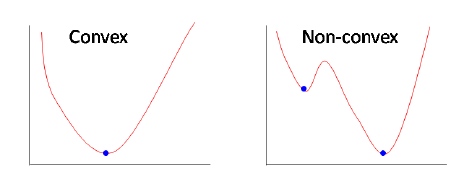
\includegraphics[scale=0.6]{convexnonconvex.png}
    \caption{Convex and Non-convex functions}
\end{figure}

Funny enough, even though most problems are non-convex, we could find a convex function that lower bounds our objective function and hope its global optimum is a decent solution to our original objective. 
Pushing this further, if we could find the tightest convex function which is a lower bound (think convex hulls), then its optimal point \emph{is} the same as our original's! 
It looks like we just turned a hard problem into a much easier one, but we unfortunately have no idea how to find this convex-hull. 
Back to square one. 

\subsection{Course Outline}

In this course, we shall deal specifically with convex optimization problems with special structure, such as: 
\itemnum
    \ii Least-Squares (LS)
    \ii Linear Programs (LP)
    \ii Convex Quadratic Program (QP)
    \ii Second-order cone programs (SOCP)
\itemend

For such specific models, very efficient solution algorithms exist with high quality implementations/software (CVX, for example). 
Most of the problems we come across can be categorized into one of the above structures, as we'll come to see. 

A large part of our time will be spent talking about affine subspaces, and normal vectors to hyperplanes to geometrically construct feasible sets. 

We'll also discuss a few non-convex problems that come up often in the real world: 
\itemnum
    \ii \emph{Boolean/integer optimization}: $x_i\in \{0,1\}^n$; some variables are constrained to be Boolean or integers. Convex optimization can be used for getting (sometimes) good approximations. 
    \ii \emph{Cardinality-constrained problems}: we seek to bound the number of non-zero elements in a vector variable. Convex optimization can be used for getting good approximations. 
    \ii \emph{Non-linear programming}: usually non-convex problems with differentiable objective and functions. Algorithms provide only local minima. 
\itemend

It goes without saying that most (but not all) non-convex problems are \emph{hard}!

For example, let's look at boolean optimization. We would like to solve $\min_{\vx} c^\T \vx$ subject to $A\vx \leq b$ and $\vx\in \{0,1\}^n$. 
One way of relaxing this into a problem that's easier to solve is to consider instead $\vx \in [0,1]^n$, i.e. going from discrete to continuous feasible set.
This is an important question because this allows us to do sparsity and feature-selection. 

What this course is for: 
\itemnum
    \ii Learning to model and efficiently solve problems arising in Engineering, Management, Control, Finance, ML, etc. 
    \ii Learning to prototype small- to medium- sized problems on numerical computing platforms. 
    \ii Learning basics of applied linear algebra, convex optimization.
\itemend

What this course is NOT: 
\itemnum
    \ii A course on mathematical convex analysis.
    \ii A course on details of optimization algorithms. 
\itemend

Here's a high level overview of what we're talking about: 
\itemnum
    \ii Linear algebra models 
    \itemnum
        \ii Vectors, projection theorem, matrices, symmetric matrices.
        \ii Linear equation, least-squares and minimum-norm problems.
        \ii Singular value decomposition (SVD), PCA, and related optimization problems. 
    \itemend
    \ii Convex optimization models 
    \itemnum
        \ii Convex sets, convex functions, convex problems. 
        \ii Optimality conditions, duality. 
        \ii Special convex models: LP, QP, SOCP.
    \itemend
    \ii Applications 
    \itemnum
        \ii Machine Learning.
        \ii Control.
        \ii Finance.
        \ii Engineering desisgn.
    \itemend
\itemend



\newpage
\section{Thursday, January 21st: Vectors and Functions}
Today's lecture went pretty fast and sped through sections, so likewise these notes are pretty rough. 
Also I don't have time to add pictures (unless I rip them off from somewhere), so I hope you have Beth Harmon level visualization powers. 

\subsection{Introduction}
We usually write vectors in column format, i.e. 
\[ x = \colvec{4}{x_1}{x_2}{\vdots}{x_n}.\] 
Element $x_i$ is the $i$th component, and the number $n$ of components is the \emph{dimension} of $x$. 
Importantly, in math, we always 1-index, not 0-index. 

We can use vectors for example in bag of words frequency matching.

\begin{example}[Time series]
    We can model a time series, i.e. the evolution of a physical or economical quantity. 
    We can represent it like $x = [x(1)\; x(2)\; \dots\; x(T)]^\T\in\RR^T$ where each $x(k)$ is the value of the quantity at time $k$.

    One example of a model for time series is an ``auto-regressive'' model, where we assume that the output depends linearly on certain previous terms and some stochasticity (i.e. error). 
    For example, if we think it only depends on the previous two days, we could write that 
    \[ x_t \approx \alpha_1 x_{t-1} + \alpha_2 x_{t-2} + \text{error}.\]
\end{example}

Vectors have a few special properties, in that the operations of sum, difference, and scalar multiplication all hold and are closed, i.e. that they return other vectors. 
These properties define a \emph{vector space}. 
The simplest example is $\Xcal = \RR^n$. 

From a vector space $\Xcal$, a nonempty subset $\mathcal{V}$ of $\Xcal$ is a \emph{subspace} if, for any scalars $\alpha, \beta$, 
\[ x,y \in \mathcal{V} \implies \alpha x + \beta y \in \mathcal{V}.\] 
For example, the set of all possible linear combinations of vectors in $S = \{x^{(1)}, \dots, x^{(m)}\}$ forms a subspace called the \emph{span} of $S$, denoted as $\spn(S)$. 

Finally, given two subspaces $\Xcal, \Ycal$ in $\RR^n$, the \emph{direct sum} of $\Xcal, \Ycal$, denoted by $\Xcal\oplus \Ycal$, is the set of vectors of the form $x+y$ with $x\in \Xcal, y\in \Ycal$. 
One can easily check that $\Xcal\oplus\Ycal$ is a subspace. 

We also have the familiar concepts of linear independence and hence the \emph{basis} for a subspace $\Scal$, the smallest set of vectors which spans $\Scal$, whose cardinality defines the dimension of the subspace.

\begin{definition}[Affine sets]
    An affine set is a set of the form 
    \[ \Acal = \{x\in \Xcal\; | x = v+x^{(0)}, v\in \Vcal\},\] 
    where $x^{(0)}$ is a given point and $\Vcal$ is a given subspace of $\Xcal$. 
    Subspaces are affine spaces containing the origin (i.e. $x^{(0)}$ is the origin). 
\end{definition}

Naturally, a \emph{line} is a one-dimensional affine set. 
We start with some point $x_0$ which hinges the line, and then some vector $v$ which determines the direction (i.e. including all multiples of it). 

Quick quiz: how many values do we need to uniquely determine lines in 2D? 
You might think it's 2, but we need to identify the vertical line as well, so it's 3. 
Think of $ax+by+c=0$. 

One question we might have is how do we measure the \emph{size} of a vector; norms are the answer to this question. 
In short, a \emph{norm} simply assigns real numbers to vectors in a consistent manner, i.e. it satisfies the following properties: 
\begin{definition}[Norm]
    A function $\|\cdot\|$ from $\Xcal$ to $\RR$ is a \emph{norm} if 
    \begin{enumerate}
        \ii $\|x\| \geq$ for all $x\in \Xcal$, and $\|x\| = 0$ iff $x = 0$; 
        \ii $\|x+y\| \leq \|x\| + \|y\|$, for any $x,y\in \Xcal$ (triangle inequality); 
        \ii $\|\alpha x\| = \alpha \|x\|$, for any scalar $\alpha$ and any $x\in \Xcal$.
    \end{enumerate}
\end{definition}

A classic example of a norm which we'll use often are the $\ell_p$ norms, defined by 
\[ \|x\|_p := \left(\sum_{k=1}^n |x_k|^p \right)^{1/p}, \quad 1\leq p < \infty.\] 

We will primarily use three norms: 
\itemnum
    \ii For $p=2$, we obtain the standard Euclidean length 
    \[ \|x\|_2 = \sqrt{\sum_{k=1}^n x_k^2},\] 
    \ii or $p=1$ which gives the sum-of-absolute-values length (or Manhattan distance) 
    \[ \|x\|_1 = \sum_{k=1}^n |x_k|.\] 
    \ii When $p=\infty$, it defines the $\ell_\infty$ norm (max absolute value norm) 
    \[ \|x\|_{\infty} = \max_{k=1,\dots, n} |x_k|.\] 
    \ii The cardinality of a vector $x$ is often called the $\ell_0$ (pseudo-) norm, which
\itemend

\subsection{Inner product}
Inner products are interesting since we can think of vectors now as functions acting on other vectors, i.e. like $\cyc{x, \cdot}$. 
\begin{definition}[Inner product]
    An \emph{inner product} on a (real) vector space $\Xcal$ is a real-valued function which maps pairs $x,y\in \Xcal$ into a scalar denoted by $\cyc{x,y}$. 
    The inner product satisfies the following axioms (for $x,y,z\in \Xcal$ and scalar $\alpha$):
    \begin{align*}
        \cyc{x,x} &\geq 0;  \\
        \cyc{x,x} &= 0 \text{ iff } x = 0;  \\
        \cyc{x+y,x} &= \cyc{x,z} + \cyc{y,z};  \\
        \cyc{\alpha x,y} &= \alpha \cyc{x,y};  \\
        \cyc{x,y} &= \cyc{y,x}.
    \end{align*}
\end{definition}

A vector space with an inner product is called an \emph{inner product space}, and the standard inner product in $\RR^n$ is the row-column product of two vectors, 
\[ \cyc{x,y} = x^\T y = \sum_{k=1}^n x_ky_k.\] 
The inner product induces a norm given by $\|x\| = \sqrt{\cyc{x,x}}$ (which you may notice is identical to the $\ell_2$-norm in $\RR^n$). 

With inner products, we can define the angle $\theta$ between two vectors $x,y$ by 
\[ \cos \theta = \dfrac{x^\T y}{\|x\|_2\|y\|_2},\]
which results from doing some easy geometry. 
This lets us characterize when $x,y$ are \emph{orthogonal} (i.e. $\theta = \pm 90^\circ$), and when $x,y$ are \emph{parallel} (i.e. $\theta = 0^\circ, \pm 180^\circ$). 

Since $|\cos\theta| \leq 1$, we easily get the following inequality. 
\begin{theorem}[Cauchy-Schwarz Inequality]
    For vectors $x,y\in \RR^n$, 
    \[ |x^\T y| \leq \|x\|_2 \|y\|_2\] 
    where equality holds when $x = \alpha y$ for scalar $\alpha$ (i.e. when $|\cos\theta| = 1$). 
    \label{thm:cs}
\end{theorem}

We also have the following generalization with $\ell_p$ norms. 
\begin{theorem}[Holder's Inequality]
    For any vectors $x,y\in \RR^n$ and for any $p,q \geq 1$ such that $1/p + 1/q = 1$, it holds that 
    \[ |x^\T y| \leq \sum_{k=1}^n|x_ky_k| \leq \|x\|_p \|y\|_q.\] 
    \label{thm:holder}
\end{theorem}

\subsection{Maximization of inner product over norm balls}
Let's solve our first optimization problem and discuss maximizing the inner product over norm balls. 
We're trying to solve the optimization problem 
\[ \max_{\|x\|_p\leq 1} x^\T y.\] 

For $p=2$, we can use the Cauchy-Schwarz inequality to get $|x^\T y\| \leq \|x\|_2 \|y\|_2$, where equality holds when $x = \alpha y$. 
Since $\|x\|_2 \leq 1$ and we want the largest positive value, we should take 
\[ x_2^* = \frac{y}{\|y\|_2},\]
so $\max_{\|x\|_2\leq 1} x^\T y = \|y\|_2$. 

For $p=\infty$, each entry of $x$ should be $\pm 1$ to satisfy the norm condition, which then maximizes the inner product by making everything positive, so 
\[ x_\infty^* = \sgn(y).\] 
So $\max_{\|x\|_\infty \leq 1} x^\T y = \|y\|_1$. 

For $p=1$, we simply set 
\[ [x_1^*] = \begin{cases} \sgn(y_i)\quad &\text{ if }i = m \\ 0 \quad &\text{ o/w } \end{cases},\quad i= 1,\dots, n,\] 
where $m$ is the index of an entry in $y$ which has maximum absolute value. 
Then $\max_{\| x\|_1 \leq 1} x^\T y = \|y\|_\infty$. 

Notice that all of these results are in line with what we'd expect by applying Holder's inequality to each case.


\subsection{Orthogonalization and Projections} 
In our favorite vector space $\RR^2$, two vectors are perpendicular when they have a dot product 0.
For generic inner product spaces, we say that two vectors $x,y$ in an inner product space $\Xcal$ are \emph{orthogonal} if $\cyc{x,y} = 0$, which we denote by $x\perp y$. 
Nonzero vectors are \emph{mutually orthogonal} if they are pairwise orthogonal.
It is a simple exercise to show that mutually orthogonal vectors are linearly independent.

Given a subset $\Scal$ of an inner product space $\Xcal$, a vector $x\in \Xcal$ is orthogonal to $\Scal$ if $x\perp s$ for all $s\in \Scal$. 
The set of vectors orthogonal to $\Scal$ is called the \emph{orthogonal complement} of $\Scal$, and is denoted by $\Scal^\perp$. 

\begin{theorem}[Orthogonal Decomposition]
    If $\Scal$ is a subspace of an inner-product space $\Xcal$, then any vector $x\in \Xcal$ can be uniquely written as the sum of an element in $S$ and an element in $S^\perp$, i.e. 
    \[ \Xcal = \Scal \oplus \Scal^\perp \quad \text{ for any subspace } \Scal\subseteq \Xcal.\]
\end{theorem}

Now we will talk about projections. 
The idea of projection is central in optimization, which is finding a point on a given set that is closest (in norm) to a given point. 

\todo{Finish writing about projections}

We have an important theorem concerning projections.
\begin{theorem}[Projection Theorem]
    \label{thm:proj}
    Let $\Xcal$ be an inner product space, $x$ be a given element in $\Xcal$, and $\Scal$ a subspace of $\Xcal$. 
    Then, there exists a unique vector $x^*\in \Scal$ which is the solution to the problem 
    \[ \min_{y\in\Scal} \|y-x\|.\] 
    Moreover, a necessary and sufficient condition for $x^*$ being the optimal solution for this problem is that $x^*\in \Scal,\; (x-x^*)\perp \Scal$. 
\end{theorem}

Let $p\in \RR^n$ be a given point. 
We want to compute the Euclidean projection $p^*$ of $p$ onto a line $L = \{x_0 + \spn(u)\}$, $\|u\|_2 = 1$. 
%For example, we can write this simply as 

Now say we want to solve the harder problem of projecting onto a span of vectors, say $\Scal = \spn(x^{(1)}, \dots, x^{(d)})\subseteq \Xcal$. 
By the projection theorem, we can convert this into a system of equations and solve. 


\subsection{Functions and maps}
In this class, we usually reserve the term \emph{function} to denote $f: \RR^n\to \RR$, and use the term \emph{map} when $f: \RR^n \to \RR^m$ and $m > 1$.

A \emph{linear} function is simply a function that perserves scaling and additivity, i.e. that 
\begin{align*}
    f(\alpha x) &= \alpha f(x) \quad\forall x\in \RR^n, \alpha\in\RR \\ 
    f(x + y) &= f(x) + f(y) \quad\forall x,y\in \RR^n.
\end{align*}

The gradient of a function can be intepreted in the context of level sets. 
Geometrically, the gradient of $f$ at a point $x_0$ is a vector $\nabla f(x_0)$ perpendicular to the contour line of $f$ at level $\alpha = f(x_0)$, pointing from $x_0$ outwards the $\alpha$-sublevel set (i.e. points towards higher values of the function). 

\newpage
\section{Tuesday, January 26th: Matrices and Linear Maps}

\subsection{Matrix Basics}
In this class, we will use the convention that if $A$ is a data matrix, then every column of $A$ is a single data point. 
Also, note that $x^\T Ay = y^\T A^\T x$, since the inner product is symmetric and the result is a scalar. 
This will be useful later on when we discuss duality. 

There's many ways we can think of a matrix-vector product. 
Let $A\in \RR^{m,n}$ with columns $a_1, \dots, a_n\in \RR^m$, and $b\in \RR^n$ a vector. 
Then we can define the product by 
\[ Ab = \sum_{k=1}^n a_k b_k,\] 
which is essentially just a weighted sum of the columns of $A$ with the elements of $b$ as coefficients. 

We can do the same definition for multiplication on the right by $A$. 
Let $\alpha_1, \dots, \alpha_m$ be the rows of $A$. 
If instead we had some $c\in \RR^m$, we can multiply on the left by it's transpose to get 
\[ c^\T A = \sum_{k=1}^m c_k\alpha_k^\T,\]
which says that this is a weighted sum of the rows $\alpha_k$ of $A$ using the elements of $c$ as coefficients. 


From matrix-vector products, we can then define matrix products.
We can view a matrix $A\in \RR^{m,n}$ in two different ways; either as a collection of columns or rows.
\[ A = \rowvec{4}{a_1}{a_2}{\dots}{a_n}, \text{   or   } A = \colvec{4}{\alpha_1^\T}{\alpha_2^\T}{\vdots}{\alpha_m^\T},\] 
where $a_1, \dots, a_n\in \RR^m$ denote the columns of $A$ and $\alpha_1^\T, \dots, \alpha_m^\T\in \RR^n$ denote the rows of $A$. 

We have three main interpretations of matrix-matrix products. 
One is obtained by letting $A$ act as a linear map on the columns of $B$, where $B = \RR^{n,p}$ and $B = [b_1\;\dots\;b_p]$. 
This gives 
\[ AB = A\rowvec{3}{b_1}{\dots}{b_p} = \rowvec{3}{Ab_1}{\dots}{Ab_p}.\] 

Similarly, we can also view the product as the linear map $B$ operating on the rows of $A$, which gives 
    \[ AB = \colvec{3}{\alpha_1^\T}{\vdots}{\alpha_m^\T} B = \colvec{3}{\alpha_1^\T B}{\vdots}{\alpha_m^\T B}.\] 

Finally, we can also write $AB$ as a sum of \emph{dyadic} matrices (i.e. rank one matrices of the form $uv^\T$).
Letting $\beta_i^\T$ denote the rows of $B$, we can write 
\[ AB = \sum_{i=1}^n a_i \beta_i^\T.\] 

\subsection{Matrices as Linear Maps}
Assume that $A$ is an $m\times n$ matrix unless stated otherwise. 
Recall that we can interpret matrices as \emph{linear maps}, i.e. maps where $f(ax+by) = af(x) + bf(y)$ for scalars $a,b$. 
Affine maps are simply linear functions plus a constant, i.e. $f(x) = Ax+b$. 

Also recall that we have the familiar concepts of range, rank, and nullspace. 
Specifically, the set of linear combinations of the columns $a_i$'s of a matrix $A$ are of the form $Ax$, for $x\in \RR^n$. 
We call this the \emph{range} of $A$, and denote it as 
\[ \Rcal(A) = \{Ax | x\in \RR^n\}.\] 
The dimension of $\Rcal(A)$ (i.e. cardinality of a basis for $A$ or the number of lin. ind. rows of $A$) is called the \emph{rank} of $A$.
We also have that $\rank(A) = \rank(A^\T)$. 

On the other hand, the null space of $A$ gives the vectors which are mapped to zero by $A$ (i.e. the \emph{kernel}) and is denoted by 
\[ \Ncal(A) = \{x \in \RR^n | Ax = 0\}.\] 

The null space of a matrix gives you the ``ambiguity'' of the solutions to $Ax = 0$. 
For any two solutions $Ax = 0$ and $Ay=0$, $A(x+y) = A(x-y) = 0$, so $x+y, x-y \in \Ncal(A)$ for example.

Importantly, $\Rcal(A^\T)$ and $\Ncal(A)$ are mutually orthogonal subspaces, i.e. $\Ncal(A)\perp \Rcal(A^\T)$, meaning that every vector in one space is orthogonal to every vector in the other.
This leads us to the following fundamental theorem. 

\begin{theorem}[Fundamental Theorem of Linear Algebra]
    For any given matrix $A \in \RR^{m,n}$, it holds that $\Ncal(A) \perp \Rcal(A^\T)$ and $\Rcal(A) \perp\Ncal(A^\T)$, hence 
    \begin{align*}
        \Ncal(A) \oplus \Rcal(A^\T) &= \RR^n \\ 
        \Rcal(A) \oplus \Ncal(A^\T) &= \RR^m.
    \end{align*}
    Consequently, we can decompose any vector $x\in \RR^n$ into a vector in the range of $A^\T$ and another in the nullspace of $A$: 
    \[ x = A^\T\xi + z, \quad z\in \Ncal(A).\] 
    Similarly, we can decompose any vector $w\in \RR^m$ into a vector in the range of $A$ and another in the nullspace of $A^\T$:
    \[ w = A\varphi + \zeta, \quad \zeta \in \Ncal(A^\T).\] 
\end{theorem}

This theorem makes much more sense geometrically. 
We did a derivation of least squares using the fundamental theorem which is cool; we revisit this anyways later on in the linear regression lecture.

\subsection{Matrix Concepts}
Things we didn't cover in lecture that I need to review and note on (for my own sake): determinants, inverses, similar matrices, eigenvalues and diagonalizability, ... 
\todo{Briefly cover eigenvalues, determinants. Similarity for spectral thm.}

Some matrices with special structure: 
\itemnum
    \ii Square, diagonal, triangular (upper or lower). 
    \ii Symmetric: a square matrix $A$ such that $A = A^\T$ (more on this later; in fact, an \emph{entire class} on it)
    \ii \textbf{Orthogonal}: a square matrix $A$ such that $AA^\T = A^\T A = I$. 
    These are interesting since this implies $A^{-1} = A^\T$. 
    So for any vector $x$, $\|Ax\|_2^2 = x^\T A^\T Ax = x^\T x = \|x\|_2^2$, so orthogonal matrices don't change the norm of $x$. 
    Hence, they actually represent rotations. 
    \ii \textbf{Dyads} (i.e. ``outer products''): matrices of the form $uv^\T$. 
    Let $A = uv^\T$. Then the $(i,j)$-th entry of $A$ is 
    \[ A_{ij} = e_i^\T(uv^\T) e_j = (e_i^\T u)(v_j^\T e_j) = u_iy_j,\] 
    (where $e_i, e_j$ are the elementary vectors) which is reminiscent of the inner product. 
\itemend

Outer products are quite useful in practice, for multiple reasons. 
If you have a data matrix like a time series, and observe that it is close to an outer product, then you can tell that you have factors which are scaled versions of each other. 

We can also find what the rank of an outer product is. 
If $A = xy^\T$, then an element of its range looks like $Az = (xy^\T)z = x(y^\T z)$. 
This last term is a scalar (as it's an inner product), so all outputs are scaled versions of $x$, and thus $A$ is rank one. 
In fact, all dyads are rank one. 

Here are some other matrix concepts that I personally find helpful.
The first is using the standard basis vectors $e_1, \dots, e_n$ to express information. 
We already saw this idea earlier when analyzing the $(i,j)$th position of the dyad $A = uv^\T$. 
If we want the $i$th row of a matrix $A$ or the $i$th entry of a column vector, we can multiply on the left by $e_i^\T$.
If we want the $j$th row of the matrix or the $j$th entry of a row vector, we can multiply on the right by $e_j$

Here's an example of where it's helpful. 
Recall from earlier that given matrices $A\in \RR^{m,n}, B \in \RR^{n,p}$, their matrix product can be written as $AB = \sum_{i=1}^n a_i \beta_i^\T$.  
If we were to insert a diagonal matrix $\diag(c_1,\dots, c_n)$ in between this product, we can break it down as 
\begin{align*}
    A \;\diag(c_1, \dots, c_n)\; B &= [A(c_1e_1)\; \dots \; A(c_n e_n)] B  \tag{using $e_1, \dots, e_n$ for the columns} \\
                                   &= [c_1 (Ae_1)\; \dots \; c_n (Ae_n)] B \\ 
                                   &= [c_1 a_1 \; \dots \; c_n a_n ] B \tag{using $a_1,\dots, a_n$ as columns of $A$}\\ 
                                   &= \sum_{i=1}^n c_i a_i\beta_i^\T \tag{using the dyadic matrix product above}
\end{align*}

In short, introducing a diagonal matrix turns this product into a weighted sum of dyads.
Useful to know for later when we discuss spectral decomposition and SVD!

\subsection{Matrix Norms}

\begin{definition}[Matrix norm]
    A function $f:\RR^{m,n}\to \RR$ is a \emph{matrix norm} if, analogously to the vector case, it satisfies three standard axioms. 
    Namely, for all $A,B\in \RR^{m,n}$ and $\alpha\in \RR$, 
    \begin{itemize}
        \ii $f(A)\geq 0$, and $f(A) = 0$ if and only if $A = 0$; 
        \ii $f(\alpha A) = |\alpha| f(A)$; 
        \ii $f(A+B) \leq f(A) + f(B)$. 
    \end{itemize}
    Many of the popular matrix norms also satisfy a fourth condition called \emph{sub-multiplicativity}: for any conformably sized matrices $A,B$, $f(AB) \leq f(A) f(B)$. 
\end{definition}

Probably the most common example of a matrix norm is the Frobenius norm.

\begin{definition}[Frobenius norm]
    The \emph{Frobenius norm} $\|A\|_F$ is simply the standard Euclidean $\ell_2$ vector norm applied to the vector formed by all elements of $A\in \RR^{m,n}$, i.e. 
    \[ \|A\|_F = \sqrt{\tr\; AA^\T} = \sqrt{\sum_{i=1}^m \sum_{j=1}^m |a_{ij}|^2}.\] 
\end{definition}
From this definition, it can also be interpreted as the sum of the eigenvalues of $AA^\T$. 

For any $x\in \RR^n$, it holds that $\|Ax\|_2 \leq \|A\|_F \|x\|_2$ (as a result of the Cauchy-Schwarz inequality applied to $|a_i^\T x|$).
Finally, the Frobenius norm is also sub-multiplicative: for any $B\in \RR^{n,p}$, it holds that $\|AB\|_F \leq \|A\|_F \|B\|_F$. 

Another type of matrix norm are the operator norms, which give a characterization of the \emph{maximum} input-output \emph{gain} of the linear map $u\mapsto Au$. 
Each choice of $\ell_p$ norm to measure the inputs and outputs in gives rise to a different norm. 
\begin{definition}[Induced Operator norm]
    The \emph{operator norm} induced by a given $\ell_p$ norm is defined as 
    \[ \|A\|_p = \max_{u\not= 0} \dfrac{\|Au\|_p}{\|u\|_p} = \max_{\|u\|=1} \|Au\|_p.\] 
\end{definition}

By definition, $\|Au\|_p \leq \|A\|_p \|u\|_p$ since $\|A\|_p$ is the max gain achieved with any choice of $u$. 
From this, it follows that any operator norm is sub-multiplicative, since for two operators $B,A$, 
\[ \|Bu\| \leq \|B\|_p \|u\|_p \implies \|ABu\|_p \leq \|A\|_p \|Bu\|_p \leq \|A\|_p\|B\|_p \|u\|_p,\]
and $\max_{\|u\|=1} \|ABu\|_p = \|AB\|_p $ by definition, so $\|AB\|_p \leq \|A\|_p \|B\|_p$. 

For the usual values of $p = 1, 2, \infty$, we have the following results (not obvious): 
\begin{itemize}
    \ii The $\ell_1$-induced norm corresponds to the largest absolute column sum 
    \[ \|A \|_1 = \max_{\|u\|_1 = 1} = \max_{j=1,\dots, n} \sum_{i=1}^m |a_{ij}|,\] 
    since $Au = u_1a_1 + \dots + u_na_n$, so maximizing the weight of the largest absolute column maximizes the norm. 
    \ii The $\ell_\infty$-induced norm corresponds to the largest absolute column sum 
    \[ \|A \|_\infty = \max_{\|u\|_\infty = 1} = \max_{i=1,\dots, m} \sum_{i=1}^n |a_{ij}|.\] 
    \ii The $\ell_2$-induced norm (sometimes called the \emph{spectral} norm corresponds to the square root of the largest eigenvalue $\la_{\max}$ of $A^\T A$: 
    \[ \|A\|_2 = \max_{\|u\|_2 = 1} \|Au\|_2 = \sqrt{\la_{\max} (A^\T A)}.\] 
    This follows from the spectral decomposition of symmetric matrices, which we'll see later.
\end{itemize}

There's also something called the \emph{spectral radius} $\rho(A) = \max_i |\la_i(A)|$ which measures the maximum modulus of the eigenvalues of $A$.
It turns out that $\rho(A) \leq \|A\|_p$ for any induced matrix norm $\|\cdot \|_p$, and that $\rho(A) \leq \min(\|A\|_1, \|A\|_\infty)$, i.e. that the radius is no larger than the maximum row or column sum of $|A|$. 

\newpage
\section{Thursday, January 28th: Matrices II}

\subsection{Orthogonalization: Gram-Schmidt}
Recall that a basis $(u_i)_{i=1}^n$ is said to be \emph{orthogonal} if $u_i^\T u_j = 0$ for $i\not= j$. 
If $\|u_i\|_2 = 1$, the basis is said to be \emph{orthonormal}.


Orthogonalization is the process where we find an orthonormal basis of the span of given vectors (which could be linearly dependent!). 
Specifically, given vectors $a_1, \dots, a_k\in \RR^n$, an orthogonalization procedures computes vectors $q_1, \dots, q_n\in \RR^n$ such that 
\[ S:= \spn \{a_1, \dots, a_k\} = \spn\{q_1,\dots,q_r\},\] 
where $r = \dim S$ and $(q_1, \dots, q_r)$ is an orthonormal basis for $S$. 

One useful concept for this process is that of a projection onto a line. 
We have a point $a\in \RR^n$ which we want to project onto a line $L(q) := \{tq : t\in \RR\}$, where $q$ is a unit vector in $\RR^n$. 
This amounts to solving the optimization problem 
\[ \min_{t\in \RR} \|a-tq\|_2\] 
for the closest point on $L(q)$ to $a$. 
The resulting vector $a_{\proj} := t^* q$ ($t^*$ being the optimal value) is this projection onto the line $L(q)$. 
This optimization problem has a simple solution (by geometry):
\[ a_{\proj} = (q^\T a) q.\] 

A simple interpretation of this is that we are \emph{removing the component} of $a$ along $q$, since $a-a_\proj$ and $a_\proj$ are orthogonal. 
Gram-Schmidt uses this idea to then create a set of vectors which are orthogonal to each other. 
The big idea is to first orthogonalize each vector w.r.t. the previous ones then normalize it to have norm one. 

\begin{theorem}[Gram-Schmidt Procedure]
    Let $a_1, \dots, a_n$ be linearly independent. 
    The Gram-Schmidt procedure below will output an orthonormal basis for $\spn\{a_1, \dots, a_n\}$. 
    \itemnum
        \ii Set $\tilde{q}_1 = a_1$. 
        \ii Normalize: set $q_1 = \tilde{q}_1/\|\tilde{q}_1\|_2.$
        \ii Remove component of $q_1$ in $a_2$:: set $\tilde{q}_2 = a_2 - (a_2^\T q_1) q_1$. 
        \ii Normalize: set $q_2 = \tilde{q}_2/\|\tilde{q}_2\|_2$. 
        \ii Remove component of $q_1, q_2$ in $a_3$: set $\tilde{q}_3 = a_3 - (a_3^\T q_1)q_1 - (a_3^\T q_2)q_2$. 
        \ii Normalize: set $q_3 = \tilde{q}_3/\|\tilde{q}_3\|_2$. 
        \ii etc.
    \itemend
\end{theorem}

We start by projecting each $a_i$ onto the previous normalized basis vectors, which makes it orthogonal to them. 
Then we normalize so that our basis becomes orthonormal.

This is well-defined, since if $\tilde{q}_i$ is ever 0, this means that the vectors are linearly dependent, which we assumed against. 
This means we can easily modify the above to produce a basis in the linearly dependent case; simply skip $a_i$ if the result $\tilde{q}_i$ turns out to be 0. 

\subsection{QR Decomposition}
The basic goal of QR decomposition is to factor a matrix as a product of two matrices which hopefully have simple structure to exploit. 
This will make it easier to solve equations $Ax = y$, since we can instead analyze $Cx = z$ and then $Bz = y$ as  
\[ Ax = B(Cx) = Bz = y.\] 
For example, if we could factor $A = BC$ where $B$ is some rotation, then we could easily solve this by taking its inverse rotation. 

The QR decomposition is just the Gram-Schmidt procedure applied to the columns of the matrix, with the result applied in matrix form. 

Consider an $m\times n$ matrix $A = (a_1, \dots, a_n)$ with columns $a_i$, and assume the columns are linearly independent. 
Then $A$ is full column-rank, so each step of G-S can be written as 
\[ a_i = (a_i^\T q_1) q_1 + \dots + (a_i^\T q_{i-1})q_{i-1} + \|\tilde{q}_i\|_2 q_i, \quad i=1,\dots, n\] 
where recall that $\tilde{q}_i = a_i - (a_i^\T q_1)q_1 - \dots - (a_i^\T q_{i-1})q_{i-1}$ (the remaining components of $a_i$, per se). 
We write this as 
\[ a_1 = r_{i1}q_1 + \dots + r_{i, i-1} q_{i-1} + r_{ii} q_i, \quad i = 1,\dots, n,\] 

where $r_{ij} = (a_i^\T q_j)$ for $1\leq j \leq i-1$ and $r_{ii} = \| \tilde{q}_i \|_2$. 

Since we got this output from G-S, we know the $q_i$'s form an orthonormal basis, so the matrix $Q = (q_1, \dots, q_n)$ satisfies $Q^\T Q = \II_n$ (i.e. is an \emph{orthonormal} matrix). 
The QR decomposition thus allows us to write the matrix in a \emph{factored} form 
\[ 
    A = QR,\quad Q = \rowvec{3}{q_1}{\dots}{q_n}, \quad R = 
    \bpm r_{11} & r_{12} & \dots & r_{1n} \\ 
         0      & r_{22} &       & r_{2n} \\ 
         \vdots &        & \ddots& \vdots \\ 
         0      &        &  0    & r_{nn} 
   \epm 
\]
where $Q$ is an $m\times n$ matrix with $Q^\T Q = \II_n$ and $R$ is $n\times n$ upper-triangular. 

With this decomposition, this makes it very efficient to solve linear equations, since any equation of the form $Ax = y$ can be written as $QRx = y$. 
We can then multiply by $Q^\T$ to get $Rx = Q^\T y$, and $R$ is upper-triangular, so we can efficiently solve this using back-substitution.


When the columns of $A$ are not independent, G-S simply skips over any zero vectors $\tilde{q}_j$ that we encounter. 
In matrix form, this means we obtain a factorization $A = QR$, with $Q \in \RR^{m\times r}$, $r = \rank(A)$, and $R$ having an upper staircase form like 
\[ R = 
    \bpm 
        * & * & * & * & * & * \\
        0 & 0 & * & * & * & * \\
        0 & 0 & 0 & 0 & 0 & * 
    \epm
\]

This is just as simple for us to solve with back-substitution, but we can also permute the columns of $R$ so that we bring all the pivot entries to thhe front. 

\subsection{Kernels in Machine Learning}
This section is quite rough since it was on the fly during lecture. We revisit this later on in the least-squares lecture, so I'd just read that section instead. 

Recall that in least-squares, our training problem is solving the optimization problem 
\[ \min_{w, b} \Lcal(X^\T w + b\cdot 1, y),\] 
where the pairs of poinits $(X_i, y_i)$ with $X_i\in\RR^n, y_i\in \RR$ form our training set.

Our predictions are then given by $\hat{y}(x) = w^\T x +  b$ once we find these optimal $w,b$.
This means we can compute an error between the \emph{actual} measured output $y_i$ with our predictions $\hat{y}_i$, which forms our loss function that we try to optimize:

\[ \min_{w,b} \sum_{i=1}^n (y_i - (w^\T x_i + b))^2.\] 

The shape of our data is $X = \rowvec{3}{x_1}{\dots}{x_m}$, i.e. an $n\times m$ matrix, so 
\[ X^\T w + b\cdot 1 = \colvec{3}{x_1^\T \cdot w + b}{\vdots}{x_m^\T \cdot w+b} .\] 
Analyzing the term $X^\T w$ is the key to understanding the impact of kernels.

Suppose we simplify our problem to 
\[ \min_w \Lcal (X^\T w) + \la \| w\|_2^2\] 
where $\la > 0$ is a penalty/regularization term on our weights trying to force our training process to find a more ``robust example for weights $w$.''
It helps account for noise in your dataset, so that small changes in the $x_i$ won't result in large changes in our loss. 

Let's analyze the simple case $m = 2$ (\# of data points) and $n = 3$ (dimension of data points). 
Invoking the fundamental theorem of linear algebra, we can write our weight vector in terms of a vector in the span of our $x_1, x_2$, i.e. $w = Xv + r$ where $v\in \spn\{x_1, \dots, x_m\}$ and $r\in \Ncal(X^\T)$, so $X^\T r = 0$. 
So $X^\T w = X^\T X v+ X^\T r = X^\T X v$, which let's us rewrite the optimization problem as 
\[ 
    \min_{w,v} \Lcal[X^\T X v, y] + \la v^\T X^\T X v.  
\]
In other words, we've converted the optimization in terms of $X$ instead into an optimization in terms of the matrix $X^\T X$. 
We refer to this matrix as the \emph{kernel} matrix $K = X^\T X$, or the Gram matrix of our data. 
Note that 
\[ K_{ij} = e_i^\T K e_j = e_i^\T X^\T X e_j = x_i^\T x_j = \cyc{x_i, x_j}.\]
This inspires us to think of other inner products that aren't just the usual scalar product $\cyc{x_i, x_j} = x_i^\T x_j$. 
We could use nonlinear products instead which let use use richer models on transformed data instead. 


\newpage
\section{Tuesday, February 2nd: Symmetric Matrices}

Today is about symmetric matrices. 
\subsection{Symmetric Matrices} 
Recall that a square $n\times n$ matrix $A$ is \emph{symmetric} if $A = A^\T$. 
The set of symmetric $n\times n$ matrices is a subspace of $\RR^{n,n}$, and is denoted by $\SS^n$. 

\begin{example}[Sample Covariance Matrix]
    \label{ex:cov}
    For one dimensional data $z_1, \dots, z_m\in \RR$, we can define the mean and variance of the data as 
    \[ \hat{z} = \frac{1}{m} \sum_{i=1}^m z_i \] 
    \[ \si^2 = \frac{1}{m} \sum_{i=1}^m (z_i-\hat{z})^2.\] 
    
    We can extend this notion to multi-dimensional points, which results in an important symmetric matrix we will see many times: the covariance matrix. 
    
    The covariance matrix is a way for us to understand the variance along any direction $u$ ($\|u\|_2=1$). 
    Let $x_1, \dots, x_m \in \RR^n$, which has sample mean $\hat{x} = \frac 1m \sum_{i=1}^m x_i$. 
    If we project our points $x$ onto this line by using $x' = (x^\T u)u$, we reduce this to the previous one dimensional case and analyze the mean and variance again.
    This creates ``scores'' of our points along the line $u$ defined by $z_i = (x_i-\hat{x})^\T u$. 
    Then following the same procedure from before, we can compute variance as 
    \begin{align*}
        \si^2(u) &= \frac{1}{m}\sum_{i=1}^m (z_i - \hat{z})^\T (z_i-\hat{z}) \\ 
                 &= \frac{1}{m}\sum_{i=1}^m u^\T (x_i-\hat{x}) (x_i-\hat{x})^\T u  \\ 
                 &= u^\T C u
    \end{align*}
    where $C= \frac{1}{m}\sum_{i=1}^m (x_i-\hat{x}) (x_i-\hat{x})^\T$ is the covariance matrix.
    From this, one can see that we can use it to compute arbitrary sample variances.
\end{example}

\begin{example}[Hessian matrix]
    The Hessian of a twice differentiable function $f: \RR^n \to \RR$ at a point $x$ is the matrix containing the second derivates of the function at that point. 
    It is given by 
    \[ H_{ij} = \dfrac{\pd^2 f(x)}{\pd x_i \pd x_j}, \; 1\leq i,j\leq n.\] 
    We usually denote the Hessian by $\nabla^2 f(x)$. 
    Since the second-derivative is the same regardless of order of derivative, $H_{ij} = H_{ji}$, so it is symmetric. 
\end{example}

As a quick aside, we can talk about quadratic functions being written in terms of matrices and vectors. 
Supposes we have a quadratic function 
\[ q(x) = x_1^2 + 2x_1x_2 + 3x_2^2 + 4x_1 + 5x_2+6,\]
which has Hessian 
\[ H = \bbm 2&2 \\ 2 & 6 \ebm.\] 

We can write the degree two monomials stricly in terms of the Hessian as 
\[ x_1^2 + 2x_1x_2 + 3x_2^2 = \frac 12 x^\T H x.\] 
Taking this further, any quadratic function can be written as the sum of a quadratic term involving the Hessian, and an affine term: 
\[ q(x) = \frac 12 x^\T H x + c^\T x + d, \quad c^\T = [4\; 5],\; d = 6.\] 

A \textbf{quadratic form} is a quadratic function with no linear and constant terms, that is $c=0, d=0$. 
Dropping the scalar, they generally look like
\[ q(x) = x^\T H x, \quad H\in \SS^n.\] 

A special quadratic form is when $H$ is diagonal, which leads to the form 
\[ q(x) = x^\T \diag(a_1, \dots, a_n) x = \sum_{i=1}^n a_i x_i^2,\] 
that is $q(x)$ is a linear combination of pure squares $x_i^2$ (i.e. no cross terms $x_i x_j$).

We can finally get to this most important result, which states that every symmetric matrix is orthogonally similar to a diagonal matrix. 

\begin{theorem}[Spectral Theorem]
    Let $A$ be a symmetric $n\times n$ matrix and let $\la_i\in \RR, (i=1, \dots, n)$ be its eigenvalues with multiplicty. 
    Then there exists a set of orthogonal vectors $u_i \in \RR^n$, $i=1,\dots, n$ such that $Au_i = \la_i u_i$. 
    Equivalently, there exists an orthogonal matrix $U = \rowvec{3}{u_1}{\cdots}{u_n}$ (i.e. $UU^\T = U^\T U = \II_n$) such that 
    \[ A = U\Lambda U^\T = \sum_{i=1}^n \la_i u_i u_i^\T, \quad \Lambda = \diag(\la_1, \dots, \la_n).\] 
\end{theorem}

In other words, $A$ can be written as the weighted sum of dyads which are mutually orthogonal. 

\todo{Write up Rayleigh quotient and matrix gain}

\subsection{Positive-Semidefinite Matrices}

\begin{definition}[Positive Semidefiniteness]
    A symmetric matrix $A\in \SS^n$ is said to be \emph{positive semidefinite} (PSD) if the associated quadratic form is nonnegative, i.e., 
    \[ x^\T A x \geq 0, \quad \forall x \in \RR^n.\]

    If, moreover, 
    \[ x^\T A x > 0, \quad \forall x\in \RR^n\setminus\{0\},\] 
    then $A$ is said to be \emph{positive definite} (PD). 
    We denote a symmetric positive semidefinite (resp. positive definite) matrix by $A\succeq 0$ (resp. $A\succ 0$). 
\end{definition}

Some immediate properties are that a PSD matrix is actually positive definite if and only if it is invertible. 
Also, it holds that 
\[ A \succeq 0 \iff \la_i(A) \geq 0,\; i=1, \dots, n.\] 
\[ A \succ   0 \iff \la_i(A) > 0,\; i=1, \dots, n.\] 

\todo{Matrix square-root, Cholesky decomp, and PSD's with ellipsoids. Maybe schur complements?}

\subsection{Principal Component Analysis}

The motivation behind PCA is that if we have a low-dimensional data set existing in a high-dimensional space, then we should instead view it from an angle where the ``variance'' of thhe data is highest. 
In other words, we want to project our data onto a direction which maximizes the resulting variance of our points, since that lets us tell the points apart the most. 

When we do this, recall that the variance of the projections of our points onto a direction $u$ is given by the covariance matrix (Example~\ref{ex:cov})
This gives us the optimization problem 
\[ \max_u\; u^\T C u: \quad \|u\|_2 = 1\] 
where $C$ is the empirical covariance matrix and we impose the unit vector constraint so that the optimization is actually tractable. 

To solve this, we can look at the spectral decomposition of $C$ given by 
\[ C = \sum_{i=1}^p \la_i u_i u_i^\T,\] 
with $\la_1 \geq \dots \geq \la_p$ and $U = [u_1,\dots, u_p]$ is orthogonal ($U^\T U = I$). Then a solution to the quadratic form 
\[ \max_{u: \|u\|_2=1} \; u^\T C u\] 
is $u^* = u_1$ where $u_1$ is the eigenvector of $C$ that corresponds to the largest eigenvalue $\la_1$ as we discussed before. 

Later we will see how to arrive at this using SVD. 


\newpage
\section{Thursday, February 4th: Singular Value Decomposition}
\todo{Add in more understandable motivation for SVD}
\subsection{The Singular Value Decomposition (SVD)}
One motivation for SVD is that we'd like to analyze data better and understand potential clusters that may arise from it. 
First, we need to understand what \emph{dyads} are. 
A matrix $A\in \RR^{m,n}$ is called a \emph{dyad} if it can be written as 
\[ A = pq^\T,\] 
for some vectors $p\in \RR^m, q\in \RR^n$, i.e. the product of a column and a row vector.
Element-wise the above reads 
\[ A_{ij} = p_iq_j, \quad 1\leq i\leq m,\; 1\leq j \leq n.\] 

Breaking this down, notice that the $j$th column of $A$ is given by 
\[A(\cdot, j) = Ae_j = q_j p,\] 
so all the columns are copies of $p$ scaled by a number, namely $q_j$. 

Similarly for the rows, the $i$th row of $A$ is 
\[ A(i, \cdot) = e_i^\T A = p_i q^\T,\] 
so the rows are scalar multiples of $q^\T$. 

The singular value decomposition theorem states that any matrix can be written as a sum of dyads with the special property that if 
\[ A = \sum_{i=1}^r p_i q_i^\T,\] 
then $p_i$ and $q_i$ are mutually orthogonal, i.e. $p_i^\T p_j = q_i^\T q_j = 0$ for all $i\not= j$. 
This special property is particularly important; it's actually really easy to write any arbitrary matrix as the sum of dyads. 
For example, we can easily break down the following matrix as 
\begin{align*}
    A &= \bbm 1 & 2 & 3 \\ 4 & 5 & 6 \ebm = \sum p_i q_i^\T \\ 
      &= 1\cdot \colvec{2}{1}{0} \rowvec{3}{1}{0}{0} + 2\cdot \colvec{2}{1}{0} \rowvec{3}{0}{1}{0} + \dots \\ 
      &= 1\cdot e_1 e_1^\T + 2e_1 e_2^\T + 3 e_1 e_3^\T + \dots.
\end{align*}

So the main contribution of SVD is that the dyads are mutually orthogonal, i.e. the $p_i$ and $q_i$ respectively are mutually orthogonal. 
It provides a three-term factorization which is similar to spectral factorization, but holds for any, possibly non-symmetric and rectangular, matrix $A$. 

\begin{theorem}[Singular Value Decomposition]
    Any matrix $A\in \RR^{m,n}$ can be factored as 
    \[ A = U \tsig V^\T = \sum_{i=1}^r \si_i u_i v_i^\T\] 
    where $U\in \RR^{m,m}$ and $V\in \RR^{n,n}$ are orthogonal matrices (i.e. $U^\T U = I_m$ and $V^\T V = I_n$), and $\tsig\in \RR^{m,n}$ is a matrix having the first $r = \rank(A)$ diagonal entries $(\si_1, \dots, \si_r)$ positive and decreasing in magnitude, and all other entries zero: 
    \[ \tsig = \bbm \Sigma & 0_{r, n-r} \\ 0_{m-r, r} & 0_{m-r, n-r} \ebm, \quad \Sigma = \diag(\si_1, \dots, \si_r) \succ 0.\]
    \label{thm:svd}
\end{theorem}
\todo{Add in proof of SVD}
Before we discuss the proof, let's analyze in further detail what SVD is really doing. 
We look at its effect as a matrix operation 
\[ x \mapsto Ax = U\tsig V^\T x.\] 
Recall that orthogonal matrices represent rotations. 
Then the operation $V^\T x =: \bar{x}$ represents a rotation of $x$, since $V^\T$ is orthogonal. 

Next, how does $\tsig$ operate on $\bar{x}$? 
It will scale some dimensions of $\bar{x}$ by the singular values, and could either crush some dimensions of $\bar{x}$ or add more. 
For example, if we have $m = 3, n = 5$, we could have the following example of crushing the dimensions $\bar{x}$:

\[ \tsig = 
\left[
\begin{array}{ccc|cc}
    1 &   &   & |  & | \\ 
      & 0.2 &   & 0  & 0 \\ 
      &   & 0 & |  & | 
\end{array}
\right], \quad 
\bar{x} = \colvec{5}{x_1}{x_2}{x_3}{x_4}{x_5} 
\implies \tsig \bar{x} = \colvec{3}{x_1}{0.2x_2}{0}.
\]

On the other hand, if $m = 5, n = 4$, we get an example of adding dimensions to $\bar{x}$.

\[ \tsig = 
\left[
\begin{array}{ccc|c}
    1 &   &   & |   \\ 
      & 0.2 &   & 0 \\ 
      &   & 0 & |    \\ \hline 
    0 & 0 & 0 & 0 \\ 
    0 & 0 & 0 & 0 
\end{array}
\right], \quad 
\bar{x} = \colvec{4}{x_1}{x_2}{x_3}{x_4}
\implies \tsig \bar{x} = \colvec{5}{x_1}{0.2x_2}{0}{0}{0}.
\]

In summary, $\tsig$ scales $\bar{x}$ and acts as a dimension adjustment. 

Since we don't care about these last few columns of $U$ corresponding to the zeroes in $\tsig$, we get a compact form of SVD. 

\begin{theorem}[Compact-form SVD]
    Any matrix $A\in \RR^{m,n}$ can be expressed as 
    \[ A = \sum_{i=1}^r \si_i u_i v_i^\T = U_r \Sigma V_r^\T, \quad \Sigma = \diag(\si_1, \dots, \si_r) \]
    where $r = \rank(A), U_r = [u_1\; \dots\; u_r]$ is such that $U_r^\T U_r = I_r$, $V_r = [v_1\; \dots\; v_r]$ is such that $V_r^\T V_r = I_r$, and $\si_1 \geq \dots \geq \si_r > 0$. 

    The positive number $\si_i$ are the \emph{singular values} of $A$, vectors $u_i$ are the \emph{left singular vectors} of $A$, and $v_i$ the \emph{right singular vectors}. These quantities satisfy 
    \begin{align}
        \label{eq:svdeig}
        Av_i = \si_i u_i, \quad u_i^\T A = \si_i v_i, \quad i = 1, \dots, r.
    \end{align}

    Morever, $\si_i^2 = \la_i(AA^\T) = \la_i(A^\T A), \; i = 1,\dots, r$, and $u_i, v_i$ are the eigenvectors of $A A^\T$ and of $A^\T A$, respectively.
\end{theorem}

Let's unpack this last statement more. 
Starting with the full form SVD of an $m\times n$ matrix $A = U \tsig V^\T$ with $U\in \RR^{m\times m}, V\in\RR^{n\times n}$, we can write out $A^\T A$ as 
\begin{align*}
    A^\T A &= (V \tsig^\T U^\T) (U \tsig V^\T) =  V \tsig^\T (U^\T U) \tsig V^\T \\ 
           &= V\tsig^\T \tsig V^\T = V \left(\begin{array}{c|c} \diag(\si_1^2, \dots, \si_r^2) & 0 \\ \hline 0 & 0 \end{array}\right) V^\T \tag{since $U$ is orthogonal}
\end{align*}

where the inside matrix is $n\times n$. 
This is the spectral decomposition of $A^\T A$, which is a symmetric matrix. 

Similarly, 
\begin{align*}
    A A^\T = U \left(\begin{array}{c|c} \diag(\si_1^2, \dots, \si_r^2) & 0 \\ \hline 0 & 0 \end{array}\right) U^\T \tag{since $V$ is orthogonal}
\end{align*}
where the inside matrix is $m\times m$. 
This is the spectral decomposition applied to the symmetric matrix $AA^\T$. 
As a result, $AA^\T \succeq 0$ and $A^\T A \succeq 0$, since all the eigenvalues are squared values and must be non-negative.

To summarize, the SVD theorem allows us to write any matrix as a sum of dyads $A = \sum_{i=1}^r \si_i u_i v_i^\T$ where the $\si_i$ provide the ``strength'' of the corresponding dyad and the rank is how many dyads we need to reconstruct $A$. 

In practice, we'll employ algorithms to compute the SVD of matrices for us.
The complexity of the algorithm which computes it via a sequence of linear transformation is $O(nm\min(n,m))$, but this can be sped up for sparse matrices if we're only interested in the largest few singular values. 

\subsection{Range and Null Space Bases via SVD}
We can infer many things from the SVD. 
For example, the rank $r$ of $A$ is the number of nonzero singular values, i.e. nonzero entries on the diagonal of $\tsig$. 

The SVD also gives us a basis for the range and nullspace of $A$.
Recall that the range of $A$ is $\Rcal(A) = \{Ax : x\in \RR^n\}$. 
We have this fundamental result relating to SVD (similar results hold for the row and left null space): 
\begin{theorem}[Column and Null Space from SVD]
Let $A\in\RR^{m,n}$ have full SVD $U\Sigma V^\T$. 
Then the first $r$ columns of $U$ give an orthonormal basis spanning the range of $A$, i.e. 
\[ \Rcal(A) = \Rcal(U_r), \quad U_r = \rowvec{3}{u_1}{\dots}{u_r}.\] 

Since $r = \rank\; A$, by the fundamental theorem the dimension of the nullspace is $n-r$. 
An orthonormal basis spanning $\Ncal(A)$ is given by the last $n-r$ columns of $V$, i.e. 
\[ \Ncal(A) = \Rcal(V_{nr}),\quad V_{nr} = \rowvec{3}{v_{r+1}}{\dots}{v_n}.\] 
\end{theorem}

These two facts are not immediately obvious, but here's some intuition. 
Special thanks to Daniel Zhu for helping out with the presented argument. 

First, we'll see why $\Rcal(A) = \Rcal(U_r)$. 
The most important step is to realize that $\Rcal(U\Sigma V^\T) = \Rcal(U\Sigma )$.
A simple argument will suffice.
If $y\in \Rcal(U\Sigma)$, then $y = U\Sigma x$. 
Now there  must be $x' \in \RR^n$ for which $Vx = x'$, so $x = V^\T x'$ and $y = U\Sigma V^\T x'$ as desired. 
The other direction is similar (in general, this holds for any invertible matrix).

Now only the first $r$ columns of $\Sigma$ are nonempty, so $\Sigma$ wipes out the last $n-r$ columns of $U$, and only the first $r$ matter. 
In equations, that means
\[ \Rcal(U\Sigma) = \left\{ U\Sigma x \;|\; x\in \RR^n \right\} = \left\{ \sum_{i=1}^r u_i \si_i x_i \;|\; x\in \RR^r \right\} = \left\{\sum_{i=1}^r u_i x'_i \; |\; x'\in \RR^r\right\} = \Rcal(U_r).\]

Here's a concrete example which might help.
Let $A$ be a $3\times 5$ matrix with entries
\[ A = \bpm 1 & 0 & 0 & 0 & 0 \\ 0 & .1 & 0 & 0 & 0 \\ 0 & 0 & 0 & 0 & 0 \epm.\] 
The rank of $A$ is clearly 2, and the range is $\Rcal(A) = \{Ax: x\in \RR^5\}$, which expands to 
\[ \left\{Ax = \colvec{3}{x_1}{.1x_2}{0} : x_1, x_2\in \RR\right\} = x_1e_1 + (.1x_2) e_2,\] 
meaning that $\{e_1, e_2\}$ is an orthonormal basis for the range.
When we add back in $V^\T$, all that happens to the basis is it gets rotated, but the range is still the same.
When we add back in $U$, $A$ selects out only the first 2 columns of $U$, so multiplying by arbitrary vector results in linear combinations of $u_1$ and $u_2$.

Now let's see why $\Ncal(A) = \Rcal(V_{nr})$.  
Using the full SVD, where $\Sigma = [s_1\; \dots\; s_n]$, we can break it down as 
\begin{align*}
    A &= U\Sigma V^\T \\ 
    AV &= U\Sigma \\ 
    \rowvec{5}{Av_1}{\dots}{Av_r}{\dots}{Av_n} &=  \rowvec{5}{Us_1}{\dots}{Us_r}{\dots}{Us_n}
\end{align*}
All the columns of $\Sigma$ after $s_r$ are empty, so $Av_i = 0$ for $i = r+1, \dots, n$. 
Since these are $n-r$ orthonormal vectors which are linearly independent and belong to $\Ncal(A)$, they must span $\Ncal(A)$.

Another similar proof (presented by Daniel) is to take $x\in \Rcal(V_{nr})$, which can be written as $x = \sum_{i=r+1}^n c_i v_i$. 
Then $Ax = \sum_{i=r+1}^n c_i (Av_i) = 0$ for the same reason as above, so $\Rcal(V_{nr})$ contains the null space, but is also dimension $n-r$, so $V_{nr}$ forms a basis.

\subsection{Matrix Norms via SVD}
\label{subsec:svd_norms}
We can also look at matrix norms using SVD. 
The \emph{squared Frobenius} matrix norm of a matrix $A\in \RR^{m,n}$ can be defined as 
\[ \|A\|_F^2 = \sum_{i,j} A_{i,j}^2 = \tr\; A^\T A = \sum_{i=1}^n \la_i (A^\T A) = \sum_{i=1}^n \si_i^2,\] 
where $\si_i$ are the singular values of $A$a. 
Hence the squared Frobenius norm is just the sum of the squares of the singular values. 

The \emph{squared spectral} matrix norm $\|A\|_2^2$, defined below, is equal to the maximum eigenvalue of $A^\T A$, so 
\[ \|A\|_2^2 = \si_1^2,\] 
i.e. the spectral norm coincides with the maximal singular value of $A$. 

The \emph{nuclear} norm of a matrix $A$ is defined as 
\[ \|A\|_* = \sum_{i=1}^r \si_i,\quad r = \rank A.\] 
This appears in problems related to low-rank matrix completion of rank minimization problems. 

We can actually prove that the squared spectral norm above is equal to the maximum eigenvalue of $A^\T A$ as follows. 
Recall that $\|A\|_2^2 = \max_{x\not= 0} \frac{\|Ax\|_2^2}{\|x\|_2^2}$, i.e. the largest matrix gain or the induced operator norm. 
Then using $A = U\tsig V^\T$,
\begin{align*}
    \|A\|_2^2 = \max_{x\not= 0} \dfrac{\|Ax\|_2^2}{\|x\|_2^2} &= \max_{x\not= 0} \dfrac{\|\tsig V^\T x \|_2^2}{\|x\|_2^2} \tag{since $U^\T U = I$} \\ 
                                                              &= \max_{z\not= 0} \dfrac{\|\tsig z\|_2^2}{\|z\|_2^2} \tag{with $z = V^\T x$} \\ 
                                                              &= \max_z \|\tsig z \|_2^2 : \quad z^\T z = 1 \\ 
                                                              &= \max_z \sum_{i=1}^r \si_i^2 z_i^2 : \quad z^\T z = 1 \\ 
                                                              &\leq \max_{1\leq i \leq r} \si_i^2,
\end{align*}
which is achieved at the largest singular value, $\si_1^2$. 
So $\si_1$ gives us a measure of how much amplification can happen multiplying by $A$.

We can use this idea to define a useful matrix property.
\begin{definition}[Condition Number]
    The \emph{condition number} of an invertible matrix $A\in \RR^{n,n}$ is defined as the ratio between the largest and the smallest singular value 
    \[ \kappa(A) = \frac{\si_1}{\si_n} = \|A\|_2\cdot\|A^{-1}\|_2.\] 
\end{definition}

The condition number provides a quantitative measure of how close $A$ is to being singular. 
The larger $\kappa(A)$ is, the more close to singular $A$ is. 

It also provides a measure of the sensitivity of the solution of a system of linear equations to changes in the equation coefficients.
Suppose we're solving the linear equation $Ax = b$ where we know there is some error $e$ in $b$. 
The condition number (roughly) gives the rate at which the solution $x$ will change with respect to a change in $b$ (i.e. error). 
More precisely, we define it to be the maximum ratio of the relative rror in $x$ to the relative error in $b$. 

Since if $A$ is nonsingular the error in the solution $A^{-1} b$ is $A^{-1} e$, the ratio above is 
\[ \frac{\|A^{-1}e\|}{\|A^{-1} b\|} / \frac{\|e\|}{\|b\|} = \frac{\|A^{-1} e\|}{\|e\|} \frac{\|b\|}{\|A^{-1} b\|}.\] 
Then the maximum such ratio is 
\begin{align*}
    \max_{e,b\not= 0} \frac{\|A^{-1} e\|}{\|e\|} \frac{\|b\|}{\|A^{-1} b\|} &= \max_{e\not=0} \frac{\|A^{-1} e\|}{\|e\|} \max_{b\not= 0}\frac{\|b\|}{\|A^{-1} b\|} \\ 
                                                                            &= \max_{e\not=0}  \frac{\|A^{-1} e\|}{\|e\|}\max_{x\not= 0}\frac{\|Ax\|}{\|x\|} \\ 
                                                                            &= \|A^{-1}\| \|A\| = \kappa(A)
\end{align*}
as we showed above.

There are other matrix properties we could derive, such as the Moore-Penrose pseudo-inverse, but we did not go over them in lecture (although I added condition number here for my own notes).

\subsection{Low-rank matrix approximation}
One problem we may consider frequently is that of approximating a matrix $A\in \RR^{m,n}$ with a matrix of lower rank. 
For example, if we have a camera taking a still video of a scene, and then a person walks by, the image matrix suddenly goes from rank 1 to nonzero rank. 
Looking for a one-rank approximation is a way we could try to remove the person from the picture. 

In particular, we consider the following rank-constrained approximation problem 
\[ \min_{A_k\in \RR^{m,n}} \|A-A_k\|_F^2\quad s.t. \rank(A_k) = k,\] 
where $1\leq k \leq r$ is given. 

Let $A = U\tsig V^\T = \sum_{i=1}^r \si_i u_i v_i^\T$ be an SVD of $A$. 
An optimal solution to the above problem is to simply truncate this summation to the first $k$ terms, i.e. take the $k$ dyads with largest singular values, 
\[A_k = \sum_{i=1}^k \si_i u_i v_i^\T.\] 

The ratio 
\[ \eta_k = \dfrac{\|A_k\|_F^2}{\|A\|_F^2} = \dfrac{\si_1^2+\dots + \si_k^2}{\si_1^2 + \dots + \si_r^2}\] 
indicates what fraction of the total \emph{variance} (Frobenius norm) in $A$ is explained by the rank $k$ approximation of $A$. 
Plotting $\eta_k$ as a function of $k$ can give helpful guidance to what $k$ would be best to approximate $A$ with. 

\begin{figure}[!htb]
    \centering
    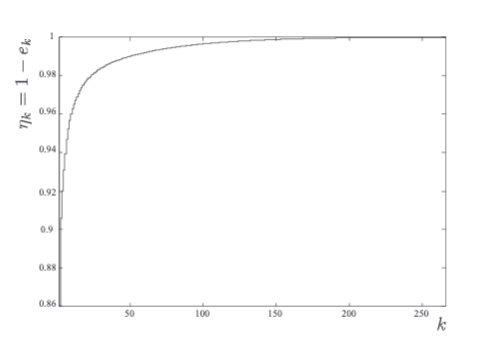
\includegraphics{lowrankappx.png}
    \caption{A plot of $\eta_k$ vs. $k$ taken from El Ghaoui's slides. Here, $k=9$ captures a good amount of variance.}
\end{figure}

\subsection{Link with PCA}
PCA is the same as low rank approximations, except you center your data first, as we'll see shortly.

Let $x_i\in \RR^n$, $i=1,\dots, m$ be the data points, so $X = \rowvec{3}{x_1}{\dots}{x_m}$.
Then replace each point with its centered version by subtracting the mean $\bar{x} = \frac 1m \sum_{i=1}^m x_i$ to get 
\[ \tilde{X} = \rowvec{3}{\tilde{x}_1}{\dots}{\tilde{x}_m}, \quad \tilde{x}_i = x_i-\bar{x}.\] 

As we discussed last lecture (see Example~\ref{ex:cov}), we want to look for a normalized direction in data space $z\in \RR^n$, $\|z||_2 = 1$, such that the variance of the projections of the centered data pointst on the line determined by $z$ is maximal. 
These components are given by $\alpha_i = \tx_i^\T z$, $i=1,\dots, m$, so the mean-square variation of the data along this direction is 
\[ \frac{1}{m} \sum_{i=1}^m \alpha_i^2 = \sum_{i=1}^m z^\T \tx_i \tx_i^\T z = z^\T \tilde{X} \tilde{X}^\T z.\] 
Hence, there's a very simple relationship between PCA and the covariance matrix $C = \frac 1m \sum_{i=1}^m (x_i-\bar{x})(x_i-\bar{x})^\T$ once you've centered the data. 

\begin{figure}[!htb]
    \centering
    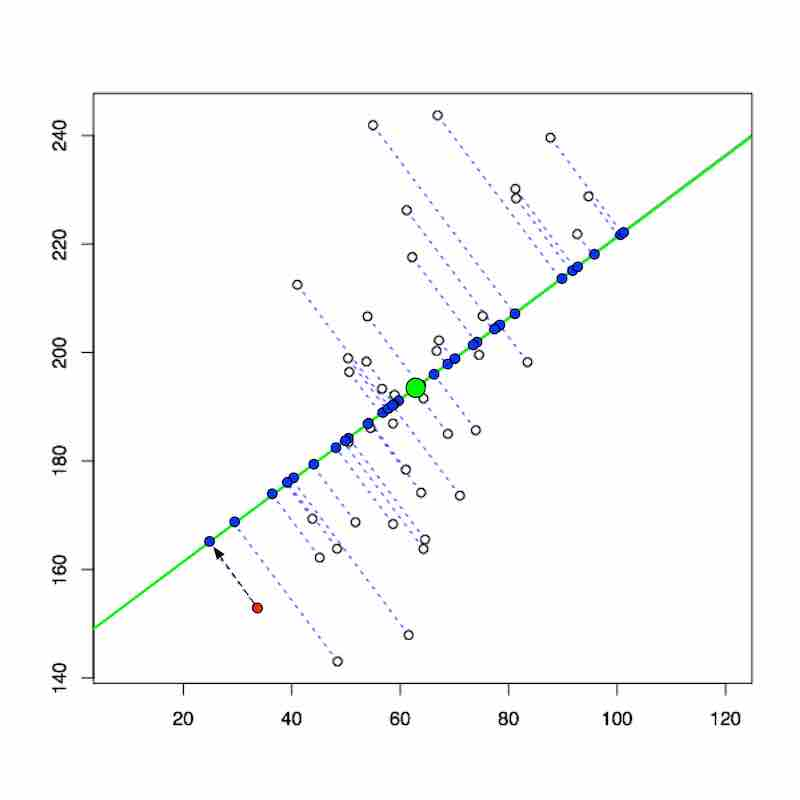
\includegraphics[scale = 0.3]{pca.jpg}
    \caption{Illustration of projecting points onto the direction $z$. Taken from Lior Pachter's blog.}
\end{figure}

Finding the maximal variance direction reduces to solving the following optimization problem: 
\[ \max_{z\in \RR^n} z^\T (\tilde{X} \tilde{X}^\T) z \quad \text{s.t. } \|z\|_2 = 1.\] 
We can directly employ SVD to solve this problem. 
Let 
\[ \tilde{X} = U_r \Sigma V_r^\T = \sum_{i=1}^r \si_i u_i v_i^\T.\] 
Then, $H = \tilde{X}\tilde{X}^\T = U_r\Sigma^2 U_r^\T$. 
We already know that this problem $z^\T H z$ is maximized by the eigenvector corresponding to the largest eigenvalue of $H$, which is $\si_1^2$.
Hence, the direction is $z = u_1$, and the mean-square variation is proportional to $\si_1^2$. 

Successive principal axes can be found by ``removing'' the first principal components and repeating these approaches on the deflated data matrix. 

In summary, there are two ways to do PCA: 
\begin{enumerate}
    \ii Form the covariance matrix $C$, find it's spectral decomposition, and take its top eigenvector (as we saw last lecture). 
    \ii Form the centered data matrix $\tilde{X}$, and find an svd of $\tilde{X} = U\tsig V^\T$.
    Then $U$ contains the eigenvectors of $C = \frac 1m \tilde{X}\tilde{X}^\T$ since $\frac 1m \tilde{X}\tilde{X}^\T = \frac 1m U\tsig^2 U^\T$ is the spectral decomposition for $C$ (as we just saw).
\end{enumerate}


\newpage
\section{Tuesday, February 9th: Linear Equations}
\subsection{Motivation for Linear Equations}
Linear equations are one of the most basic form of relationship among variables in an engineering problem. 
There's all sorts of applications of linear equations that come up in science, and they form the building block for many other optimization methods, so it's important to know how to solve them.

Here is an example of a system in 3 equations in 2 unknowns: 
\begin{align*}
    x_1 + 4.5x_2 &= 1 \\ 
    2x_1 + 1.2x_2 &= -3.2  \\
    -0.1x_1 + 8.2x_2 &= 1.5.
\end{align*}

We can write this in vector format as $Ax=y$, where 
\[ A = \bbm 1 & 4.5 \\ 2 & 1.2 \\ -0.1 & 8.2 \ebm, \quad y = \colvec{3}{1}{-3.2}{1.5}.\] 
Solutions are $x\in \RR^2$ which satisfy the equation. 
In this case, the equation has no solution, i.e. the system is \emph{infeasible}.

We then went over a lot of examples. 
I prefer theory so I did not take notes on them.

\subsection{Set of Solutions of Linear Equations}
Our general setup is that we want to solve the linear equation 
\[ Ax = y, \quad A \in \RR^{m,n}.\] 

There are many issues we concern ourselves with, such as existence and uniqueness of solutions, or the characterization of the \emph{solution set} 
\[ S = \{x\in \RR^n : Ax=y\}.\] 
Notice that $Ax$ always lies in $\Rcal(A)$, so $S\not= 0 \iff y \in \Rcal(A)$. 
Hence, there is a solution if and only if $\rank([A\; y]) = \rank(A)$. 

When existence is satisfied, the set of solutions is the affine set 
\[ S = \{\bar{x} + Nz, z\in \RR^{n-r} \},\] 
where $\bar{x}$ is any vector such that $A\bar{x} = y$, $r = \rank(A)$, and $N \in \RR^{n, n-r}$ is a matrix whose columns span the nullspace of $A$ (hence $AN = 0$). 

Geometrically, the null space represents the span of the ``free variables'' in the solutions.

Finding the solution set in the above manner can be useful in optimization. We can use this by turning our usual optimization problem into an unconstrained one, i.e. 
\[ \min_x f_0(x) :\; Ax = b \implies \min_z f_0(x_0 + Nz),\] 
using notation from above. 

\subsection{Solving Linear Systems}
We can also use SVD to easily analyze our linear equation system.
As usual, suppose we're solving $Ax = y$ where $A\in \RR^{m,n}$ and $y\in \RR^m$. 
If $A = U\tilde{\Sigma} V^\T$ is the SVD of $A$ (see Theorem~\ref{thm:svd}), then $Ax = y$ is equivalent to 

\[ U\tilde{\Sigma} V^\T x = y \implies \tilde{\Sigma} V^\T x = U^\T y \implies \tilde{\Sigma} \tilde{x} = \tilde{y},\] 
where $\tilde{x} = V^\T x, \tilde{y} = U^\T y$. 

In other words, we're using $U$ and $V$ to rotate our inputs and outputs to make the system diagonal (as per the usual SVD interpretation). 
Since $\tilde{\Sigma}$ is a diagonal matrix 
\[ \tilde{\Sigma} = \bbm \Sigma & 0_{r, n-r} \\ 0_{m-r, r} & 0_{m-r, n-r} \ebm,\quad \Sigma = \diag(\si_1, \dots, \si_r) \succ 0,\]

this makes the system very easy to solve or analyze.
Note that $\Ncal(A) = m-r$. 

Let's analyze the resulting system $\tilde{\Sigma}\tilde{x} = \tilde{y}$, which reduces to 
\begin{align*}
    \si_i \tilde{x}_i &= \tilde{y}_i \quad i = 1, \dots, r \\ 
    0 &= \tilde{y}_i \quad i = r+1, \dots, m.
\end{align*}

Clearly we need $\tilde{y}_i$ to be zero for its last $m-r$ components, which happens when $y\in \Rcal(A)$. 
Otherwise the solution set is empty. 

If $y\in \Rcal(A)$, then we can solve for $\tilde{x}$ with our first set of conditions: $\tilde{x}_i = \tilde{y}_i/\si_i$ for $i = 1, \dots, r$, with the last $n-r$ components being free (which correspond to elements in the nullspace of $A$).

When $A$ is full column rank, it has trivial nullspace and hence there is a unique solution. 

\begin{example}
    Suppose we have a system $Ax = y$ with 
    \[ A = \bbm \si_1 & 0 & 0 \\ 0 & \si_2 & 0 \\ 0&0&0 \\ 0&0&0\ebm, \quad y=\colvec{4}{y_1}{y_2}{y_3}{y_4}.\]
    This system has no solution if $(y_3, y_4) \not= 0$. If $y_3=y_4 = 0$ so that $y\in \Rcal(A)$, we then get the solution sest $S = \{x_0 + Nz : z\in \RR^2\}$ with 
    \[ x_0 = \colvec{4}{y_1/\si_1}{y_2/\si_2}{0}{0},\quad N = \bbm 0&0\\0&0\\1&0\\0&1\ebm.\] 
\end{example}

Finally, we can also use QR decomposition to analyze a linear system. 
The idea is to reduce the system to a triangular one and then solve using ``back-substitution.'' 
For example, if $A$ is square and $A = QR$ with $Q^\T Q = I_n$, then $Ax = y$ is equivalent to $Rx = \tilde{y} = Q^\T y$, which is triangular. 
Then we just have to back substitute to find a solution. 

Similarly to using SVD, we're rotating our outputs here to make the system triangular and easier to solve.

\newpage

\section{Thursday, February 11th: Least-Squares and Variants}
\subsection{Ordinary Least-Squares and Minimum-Norm Solutions}
One classical \textbf{goal} of modeling is the following: given $A\in \RR^{m\times n}, y\in \RR^m$, find $x$ such that $Ax \approx y$. 
In other words, if $A = [a_1 \;\dots\; a_n]$, then we are asking if $y$ can be written as the linear combination of the columns of $A$, i.e. $y \approx \sum_{i=1}^n x_i a_i$. 

The least squares approach uses the Euclidean norm to rate our approximation, solving the optimization problem 
\[ \min_x \|Ax - y\|_2.\] 
Since the objective function is always $\geq 0$, we can solve the ``ordinary least-squares'' problem 
\[ \min_x \|Ax-y\|^2_2 = \sum_{i=1}^m r_i^2, \quad r := Ax-y,\] 
i.e. minimizing the sum of squared residuals. 

Geometrically, since $Ax\in \Rcal(A)$, the problem amounts to finding the point $\tilde{y} = Ax^*$ in $\Rcal(A)$ at \emph{minimum distance} from $y$. 
By the Projection Theorem (Theorem~\ref{thm:proj}), this is just the orthogonal projection of $y$ onto the subspace $\Rcal(A)$.
Notice the similarity to projections on a line, where we minimize $\|ax-y\|_2^2$ for a single vector. 

Another interpretation of this problem can be in terms of the rows $a_i^\T$ of $A$, as we were alluding to above. 
The problem then becomes 
\[ \min_x \; \sum_{i=1}^m (y_i - a_i^\T x)^2.\] 
Here, we're trying to fit every component $y_i$ as some linear combination of the input $a_i$, where $x$ determines the coefficients. 

This interpretation hails from machine learning, where this is often useful for prediction. 
We have some training set where we find what the solution $x^*$ to the above problem is, and then we can predict the output corresponding to a new vector $a\in \RR^n$ (a \emph{test point}) by computing $\hat{y} = a^\T x^*$. 

We usually write least-squares in the above form because it leads us to an easy proof of the closed-form solution. 
As $y-Ax^* \in \Rcal(A)^\perp = \Ncal(A^\T)$, we have $A^\T (y - Ax^*) = 0$. 
This leads us to the following result. 

\begin{theorem}[Closed-Form Least Squares]
Any solution to the least-squares problem must satisfy the \textbf{Normal Equations} 
    \[ A^\T Ax = A^\T y.\] 
This system always admits a solution, and if $A$ is additionally full column rank, then the solution is unique and is given by 
\[ x^* = (A^\T A)^{-1} A^\T y.\] 
\end{theorem}
Recall that $A^\T A$ is invertible since if it is full rank, $\|Ax\|_2^2$ is never 0 if $x\not= 0$, so $x^\T A^\T A x > 0$ meaning $A^\T A$ is positive definite. 

As a corollary, notice that the set of optimal solutions is 
\[ \Xcal_{\opt} = A^\dagger y + \Ncal(A),\] 
where $A^\dagger y$ is the minimum norm point in the optimal set. 
Adding anything from the null space will still make it a solution that is optimal, just not necessarilly minimum norm. 

We can also find solutions of OLS via QR decomposition. 
Assume the columns of $A\in \RR^{m\times n}$ are linearly independent so that the QR factorization $A = QR$ exists, with 
\begin{itemize}
    \ii $m\times n$ matrix $Q$ satisfies $Q^\T Q = I$, 
    \ii $n\times n$ matrix $R$ invertible,
    \ii then $A^\dagger = (A^\T A)^{-1} A^\T = R^{-1} Q^\T$.
\end{itemize}
This gives us the following algorithm.
\begin{itemize}
    \ii compute the QR factorization of $A = QR$ ($2mn^2$ flops);
    \ii form $z = Q^\T y$ ($2mn$ flops); 
    \ii solve the triangular system $Rx = z$ via backward substitution. 
\end{itemize}

In total, our algorithm is identical for solving $Ax = b$ for square invertible $A$ and has complexity is $2mn^2$ flops.

\subsection{Variants of Least-Squares}
A generalization of the basic LS problem allows for the addition of linear equality constraints on $x$, resulting in the constrained problem 
\[ \min_x \|Ax - y\|_2^2,\quad \text{s.t. } Cx = d,\] 
where $C\in \RR^{p,n}$ and $d \in \RR^p$. 

This may look difficult to solve now, but we can convert it into a standard LS problem by ``eliminating'' the equality constraints via a standard procedure. 
Assume the problem is feasible, and let $\bar{x}$ be such that $C\bar{x} = d$, and let $N$ have columns which are a basis for $\Ncal(C)$. 
Then all of the feasible points can be expressed as $x = \bar{x} + Nz$, so our unconstrained problem in the variable $z$ becomes 
\[ \min_z \|\bar{A} z - \bar{y} \|_2^2,\] 
where $\bar{A} = AN, \bar{y} = y - A\bar{x}$. 

Another variant is \emph{Weighted Least-Squares}, where we want to give different weights to our residuals, instead minimizing $f_0(x) = \sum_{i=1}^m w_i^2 r_i^2$ where $w_i\geq 0$ are the given weights. 
We can easily convert this as 
\[ f_0(x) = \|W(Ax - y)\|^2_2 = \|A_w x - y_w \|_2^2,\] 
where $W = \diag (w_1, \dots, w_m)$, $A_w = WA$, and $y_w = Wy$. 
This is again our original LS problem with row-weighted matrix $A_w$ and vector $y_w$. 

One popular variant of LS is the class of regularized LS problems, which are of the form 
\[ \min_x\; \|Ax - y\|_2^2 + \phi(x),\] 
where a ``regularization,'' or \emph{penalty} term $\phi(x)$ is added to our usual LS objective. 
Typically $\phi(x)$ is proportional to either the $\ell_1$ or $\ell_2$ norm of $x$. 
In the former case, the problem is known as LASSO. 
We will instead discuss the latter case, known as \emph{ridge regression}. 

Consider the problem 
\[ \min_x \; \|Ax - y\|_2^2 +\la\|x\|_2^2, \quad \la \geq 0.\] 
We can use the fact that the squared $\ell_2$ norm of block vectors is the sum of the squared norms of the blocks to rewrite our problem as 
\[ \|Ax-y\|_2^2 + \la \|x\|_2^2 = \|\tilde{A}x - \tilde{y}\|_2^2,\] 
where 
\[ \tilde{A} = \colvec{2}{A}{\sqrt{\la} I_n}, \quad \tilde{y} = \colvec{2}{y}{0_n}.\] 
By construction $\tilde{A}$ is full column rank due to the $I_n$. 
Here, $\la\geq 0$ is a tradeoff parameter between output accuracy and input effort. 
Since $\la$ is a hyperparameter, we typically try out a bunch of different values to find the one with the best test accuracy on unseen data. 

Applying our solution from above, we find that the optimal solution is just 
\[ x^* = (A^\T A + \la I_n)A^\T y,\] 
which always exists and is unique since $\tilde{A}$ is always full column rank. 

\subsection{Kernels for Least-Squares}
Before we talk about kernel learning, we're going to try and motivate it. 
Suppose we're making a nonlinear auto-regressive model for time-series, where $y_t$ is a \emph{quadratic} function of $y_{t-1}$ and $y_{t-2}$. 
This can be modeled by 
\[ y_t = w_1 + w_2 y_{t-1} + w_3y_{t-2} + w_4 y^2_{t-1} + w_5 y_{t-1}y_{t-2} + w_6 y_{t-2}^2.\] 
We can't exactly model this by a LS formulation with just $x_t = \rowvec{2}{y_{t-1}}{y_{t-2}}^\T$, but if we augment our data with a function $\phi(x_t)$, where 
\[ \phi(x_t) := (1,y_{t-1}, y_{t-2}, y^2_{t-1}, y_{t-1}y_{t-2}, y^2_{t-2}),\] 
then we can write it as $y_t = w^\T \phi(x_t)$. 
Thus, we can just solve the classic LS problem 
\[ \min_w \sum_{t=1}^T (y_t - w^\T \phi(y_t))^2,\] 
where our model is nonlinear in the data, but is linear in the model coefficients. 
If it was nonlinear in the coefficients, this would be a neural network. 

With this realization, we can create non-linear (e.g. quadratic) decision boundaries, such as 
\[ w_1x_1 + w_2x_2 + w_3x_1^2 + w_4 x_1x_2 + w_5x_2^2 = b = 0.\]
This can be written as $w^\T \phi(x) + b = 0$ where $\phi(x) := (x_1, x_2, x_1^2, x_1x_2, x_2^2)$. 

\begin{figure}[!htb]
    \centering 
    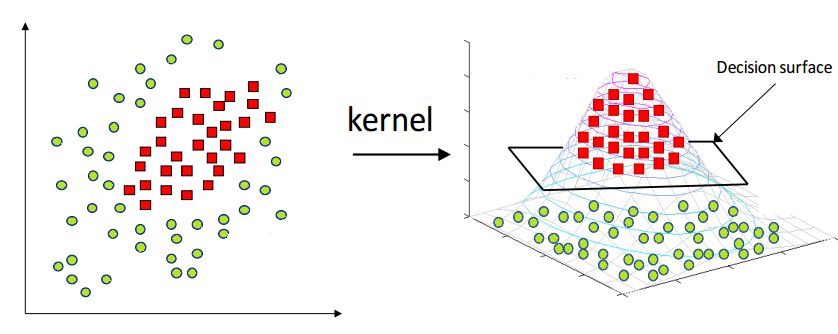
\includegraphics[scale=0.35]{kernel.png}
    \caption{An example of moving to a higher dimension to create a linear decision boundary separating the data. Image taken from \href{https://medium.com/@zxr.nju/what-is-the-kernel-trick-why-is-it-important-98a98db0961d}{this medium article by Grace Zhang}.}
\end{figure}

If we can do this, then in theory it seems we could always augment our input with enough dimensions to make any data separable. 
The question is how to do this in a computationally feasible manner. 

First, let's look at the regularized learning setting for inspiration.  
The setup is to find
\[ w^* = \min_w \|X^\T w - y\|^2_2 + \la \|w\|^2_2\] 
where 
\begin{itemize}
    \ii $X = [x_1, \dots, x_n]$ is a $p\times n$ matrix of data points,
    \ii $y\in \RR^n$ is the response vector (or labels), 
    \ii $w\in \RR^p$ is the classifier or regression coefficients, 
    \ii $\la\geq 0$ is a regularization parameter. 
\end{itemize}

With the optimal coefficients $w^*$, prediction simply requires computing $\hat{y} = (w^*)^\T x$ where $x\in \RR^p$ is a new data point. 

In general, the key result is that for any generic problem 
\[ \min_w \Lcal(X^\T w, y) + \la \|w\|_2^2\] 
where $\Lcal$ is any loss function, the optimal $w$ lies in the span of the data points $(x_1,\dots, x_n)$, i.e. $w = Xv$ for some $v\in\RR^n$. 
In the above problem, we used $\Lcal(z,y) = \|z-y\|^2_2$, i.e. the squared $\ell_2$-norm. 
\begin{proof}
    Invoke the fundamental theorem of linear algebra, and write $w\in \RR^p$ as the sum of two orthogonal vectors, one in the range of $X$ and another orthogonal to it. 
    Then
    \[ w = Xv + r,\]
    where $v\in \RR^n$ and $X^\T r = 0$ (since $r\in \Rcal(X)^\perp = \Ncal(X^\T)$).
    Applying this to our problem above and instead minimizing over $v$ and $r$ gives 
    \[ \min_{v,r} \Lcal(X^\T (Xv+r), y) + \la (\|Xv+r\|_2^2) = \min_{v,r} \Lcal(X^\T Xv, y) + \la (\|Xv\|^2_2+\|r\|_2^2) ,\] 
    where we used the Pythagorean theorem in the last step since $Xv$ and $r$ are orthogonal. 
    Hence, setting $r = 0$ is optimal, and hence $w = Xv$ as we claimed.
\end{proof}

Using this result, we can show that our training problem rewrites as 
\[ \min_v \Lcal(Kv, y) + \la v^\T K v\]
which depends only on the $n\times n$ (PSD) ``kernel'' matrix $K := X^\T X$. 
Note that 
\[ K_{ij} = x_i^\T x_j, \quad 1\leq i,j\leq n,\] 
that is, $K$ contains the scalar products between all data point pairs. 

Now, our prediction/classification rule depends solely on the scalar products between any new point $\tilde{x}$ and our training data points $x_1, \dots, x_n$. 
Since $w = Xv$, we have
\[ w^\T \tilde{x} = v^\T X^\T \tilde{x} = v^\T k, \quad \text{ where } k := X^\T \tilde{x} = (x_1^\T \tilde{x},\dots, x_n^\T \tx).\]

Note the computational advantage here! 
Once $K$ is formed (this takes $O(n^2p)$), then the training problem only has $n$ variables. 
When $p \gg n$, this leads to a dramatic reduction in problem size.

We haven't touched upon how this lets us create a richer class of models yet, so let's revisitt that. 
In the nonlinear case, we can replace the feature vectors $x_i$ by some ``augmented'' feature vectors $\phi(x_i)$, with $\phi$ a non-linear mapping. 

For example, recall in classification with a quadratic decision boundary, we optimized 
\[ \min_w \sum_{i=1}^n (y_i - \phi(x_i)^\T w)^2 \text{  where  } \phi(x) := (x_1, x_2, x_1^2, x_1x_2, x_2^2). \]
This leads to the modified kernel matrix 
\[ K_{ij} = \phi(x_i)^\T \phi(x_j), \; 1\leq i,j\leq n,\]
which, like the old kernel matrix, gives us scalar products between data points, except now the points are augmented. 

Since we only need to know the scalar products, actually all we need is the \emph{kernel function} associated with mapping $\phi$, which is 
\[ k(x,z) = \phi(x)^\T \phi(z).\] 
It gives us information about the metric in the feature space, e.g. 
\[ \| \phi(x) - \phi(z) \|^2_2 = k(x,x) - 2k(x,z) + k(z,z).\] 
However, this function $k(\cdot, \cdot)$ can't be constructed arbitrarily; it has to satisfy our above condition for some $\phi$. 

Finally, suppose we have two different augmented points $\phi(x)$ and $\phi(z)$ for some given two vectors $x,z\in\RR^2$.
Then it turns out (and is easily verified upon inspection) that  
\[ k(x,z) = \phi(x)^\T \phi(z) = (1 + x^\T z)^2.\] 
So instead of needing to expand $\phi(x)$ which is an expensive operation scaling exponentially, we can instead just work with this dot product formula which is more efficient (i.e. linear in the dimension of our vectors, in this case 2).  

More generally, when $\phi(x)$ is the vector formed with all the products between the components of $x\in \RR^n$ up to degree $d$, then for any two vectors $x,z\in \RR^n$, 
\[ \phi(x)^\T \phi(z) = (1+x^\T z)^d.\] 
Our computational effort grows linearly in $n$ since we just need to form this dot product. 

Compare this with the ``brute force'' approach, where we first form $\phi(x),\phi(z)$ and then evaluate $\phi(x)^\T \phi(z)$. 
Here, the computational effort grows as $n^d$! 
In other words, we found a way to reduce an exponential effort to a linear one; pretty good I'd say. 

This is what most people will refer to as the \emph{kernel trick}, which allows us to pseudo-augment our data points into infinite-dimensional spaces. 
For example, we could also consider using the Gaussian kernel function (radial basis function) 
\[ k(x,z) = \exp \left(-\dfrac{\|x-z\|^2_2}{2\si^2}\right),\] 
where $\si>0$ is a scale parameter. 
In order to approximate this kernel function by some $\phi$, we'd need to use a series for the exponential that goes on infinitely, i.e. $\phi$ is mapping into an infinite-dimensional space. 

\newpage
\section{Tuesday, February 16th: Linear Algebra Review}
Today is a linear algebra review for the quiz on Thursday.

Recall that projections are solving the optimization problem where given a point $x$, and some line going through $x_0$ in the direction of $v$ ($\|v\|_2 = 1$), we want to find the point $z$ on that line closestt to $x$. 
The line is defined by $\Lcal = \{x_0 + tv : t\in \RR\}$, and our optimal $z$ will look like $z = x_0 + t^* v$. 
The problem to be solved is 
\[ \min_t \|x_0 + tv - x\|_2^2.\] 
To solve this, we expand the objective as 
\[ (x_0+tv - x)^\T (x_0 + tv - x) =  t^2 v^\T v + 2tv^\T (x_0-x) + (x_0-x)^\T (x_0 - x) ,\]
and go about optimizing with gradients. 
Using $v^\T v$, the optimal value of $t$ simplifies to $t^* = v^\T (x-x_0)$, i.e. the scalar product between $v$ and $x-x_0$ as expepcted. 
This is one of the most important optimization problems to know, which is why we've gone over it so many times.

Hyperplanes are also very important to understand. 
Suppose we have the plane $\{x: a^\T x = b\}$, and we want to project $0$ onto the hyperplane, i.e. find the closest point to 0.
We can rewrite this by first finding an $x_0$ for which $a^\T x_0 = b$, $x_0\not= a$. 
We know that $x_0 = \alpha a$ (by the fundamental theorem of linear algebra), so 
\[ \alpha a^\T a = b \implies \alpha = \frac{b}{\|a\|_2^2},\; x = \frac{ba}{a^\T a}.\]

The rest of today was review of previous days, so I didn't take notes.

\newpage
\section{Tuesday, February 23rd: Linear Programs}
We're starting the next portion of the course, which will be focused on ``conic optimization.'' 
The main motivation comes from some problems which we've already seen can be solved by SVD/PCA, such as 
\begin{itemize}
    \ii $\min_{X} \|Ax-y\|_2^2 + \la \|x\|_2^2$ for $\la > 0$ (Ridge Regression)
    \ii $\min_{L,R} \|X-LR^\T\|_F^2$ where $L, R$ have $k$ columns ($k < \min(n,m)$). 
\end{itemize}

Our goal will be to discuss an entire class of optimization problems called conic optimization, which will lead us into discussing linear programming.

\subsection{Polyhedrons}
To talk about linear programs, we first need to discuss the geometry of the set of points we want to work with. 
For a given $a\in \RR^n$ and $b\in \RR$, the set $\Hcal$ of points satisfying the linear inequality $a^\T x \leq b$ is a closed half-space. 
Its boundary is the hyperplane defined by the \emph{equality} $a^\T x = b$. 

The way to think about this is to start with the boundary $a^\T x=0$, which is simply the plane normal to $a$ passing through the origin. 
Then if $\Hcal = \{x\; |\; a^\T x \leq 0\}$, then $\Hcal$ is the set of points forming an obtuse angle with $a$ (by properties of inner products). 

\vspace{.4cm}
\begin{minipage}{.4\textwidth}
    \centering
    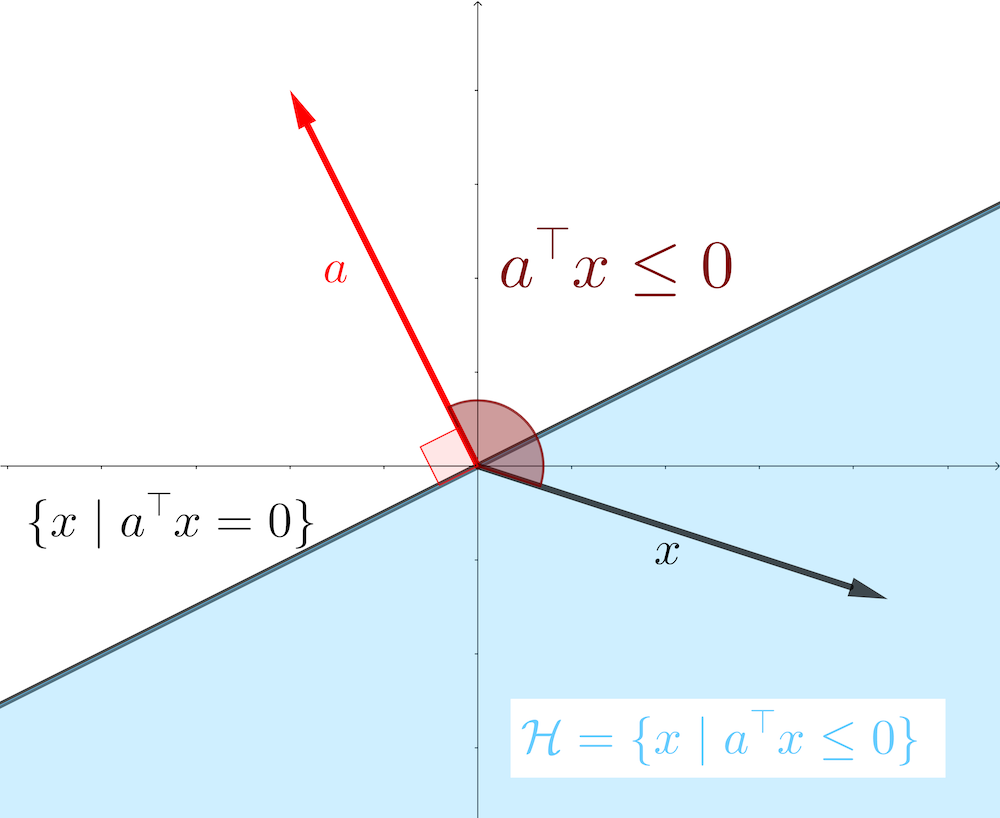
\includegraphics{hp0.png}
    \captionof{figure}{The half-space $a^\T x \leq 0$.}
\end{minipage}%
\begin{minipage}{.6\textwidth}
    \centering
    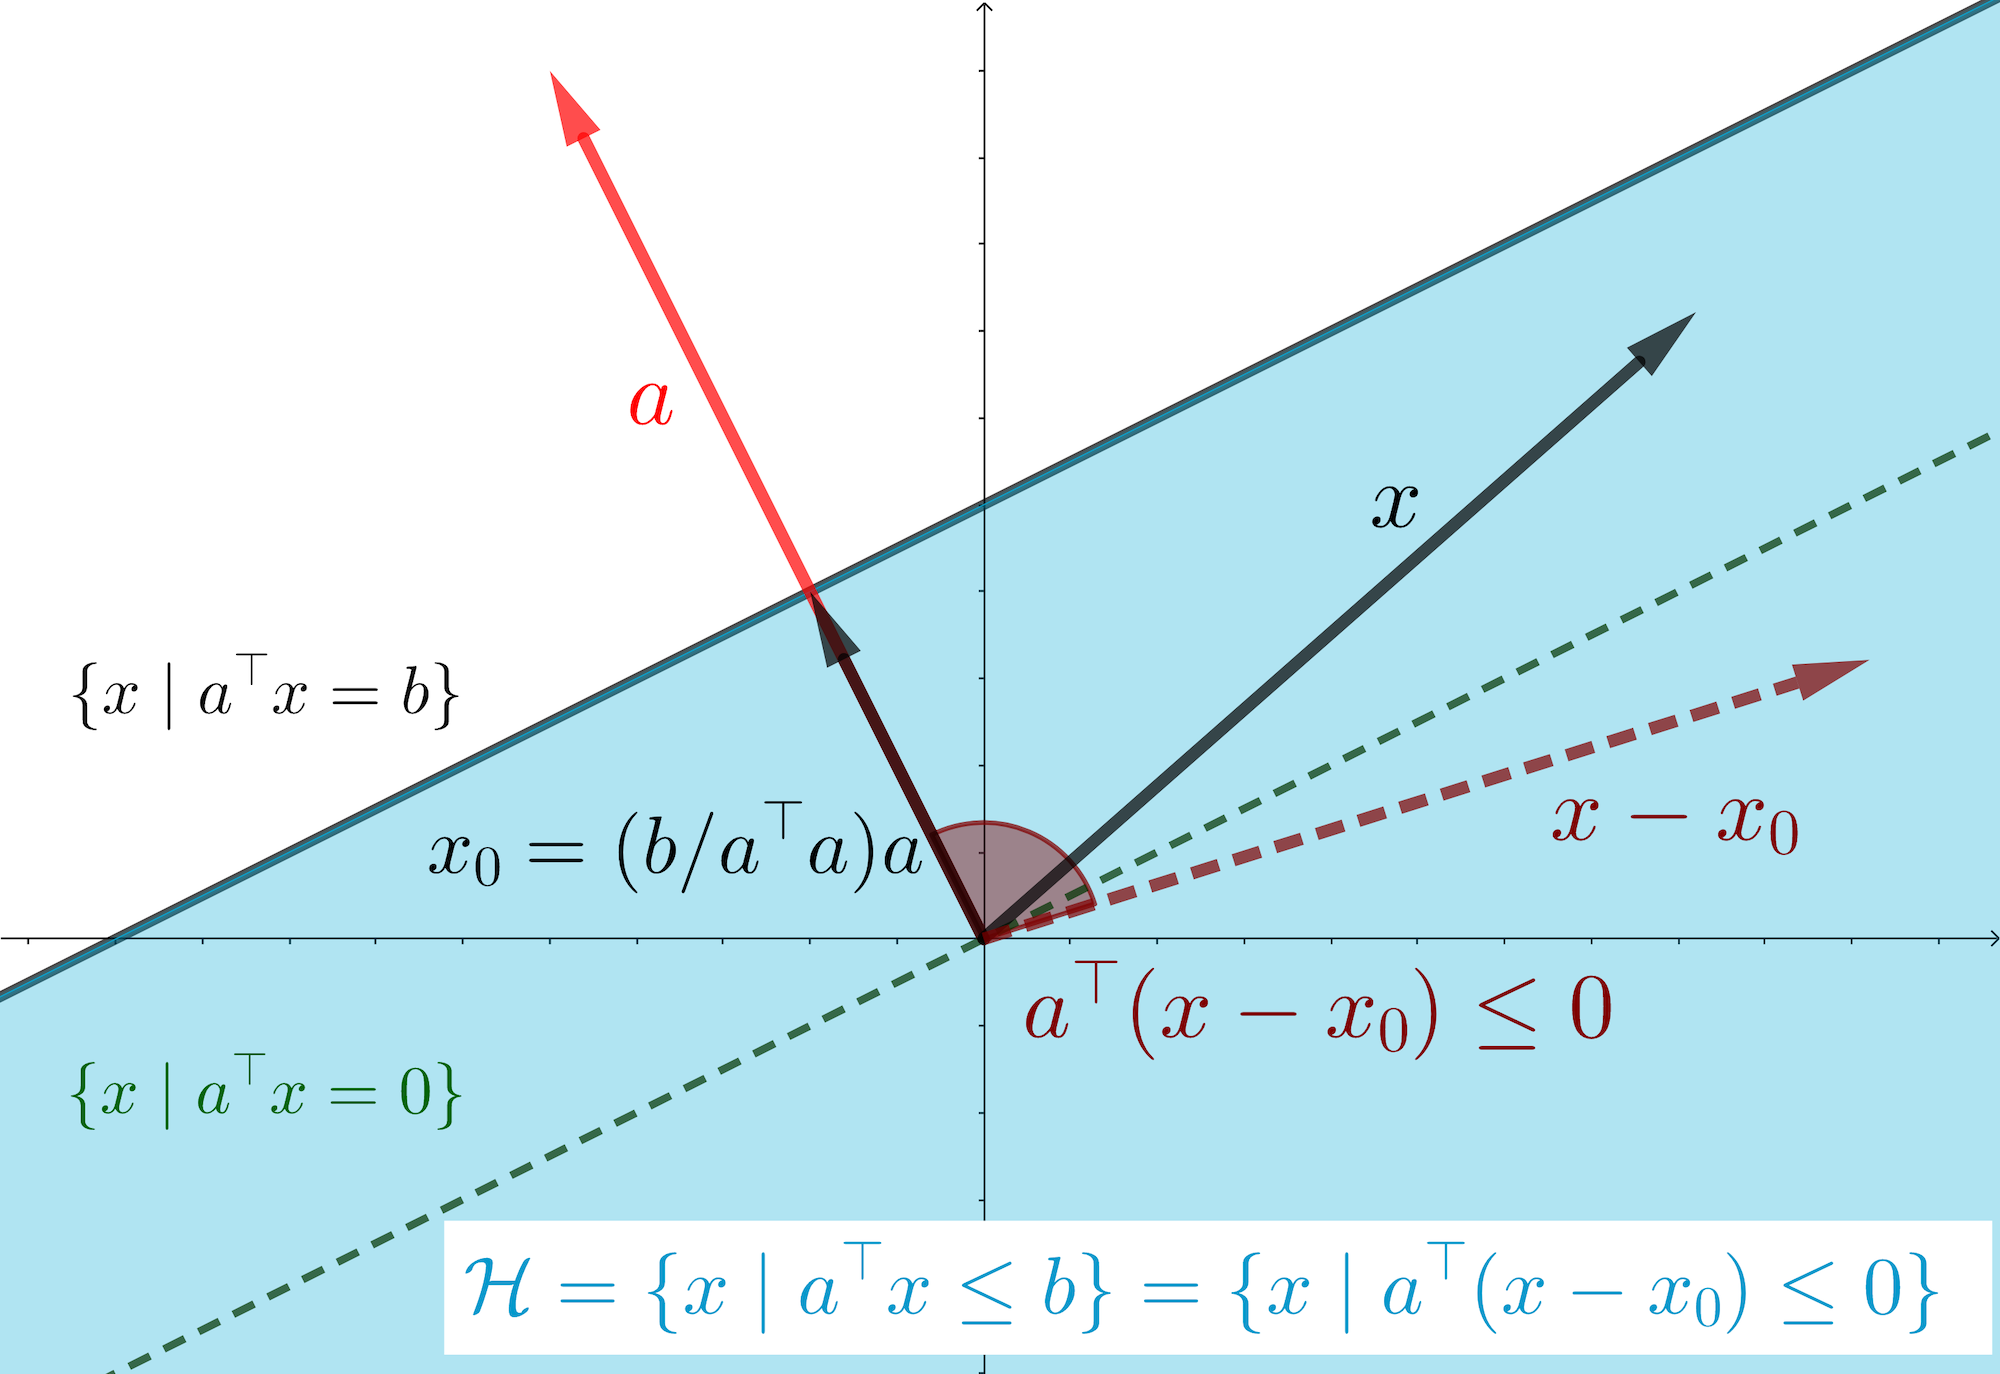
\includegraphics[scale=0.75]{hpb.png}
    \captionof{figure}{The half-space $a^\T x \leq b$ (figures my own).}
\end{minipage}%
\vspace{.4cm}

Now if we consider $a^\T x \leq b$, our boundary plane instead passes through the point $x_0 = (b/a^\T a) a$ (see the previous lecture), so the value $b$ just tells us how far along $a$ the boundary sits. 

We can interpret this half-space as being the set of points whose inner product with $a$ is less than $b$ (obviously), which occurs below the boundary. 
However, a more illuminating intepretation is to rewrite the half-space as $a^\T x - b = a^\T (x-x_0) \leq 0$, which reduces to the case we just had. 
Hence the desired region is the one from before but shifted in the direction of $a$ by $x_0$. 


For given $a_1, \dots, a_m\in \RR^n$, and $b\in \RR^m$, the collection of $m$ linear inequalities 
\[ a_i^\T x \leq b_i, \quad i = 1,\dots, m\] 
defines a region in $\RR^m$ which is the intersection of $m$ half-spaces and it is named a \emph{polyhedron}. 
Depending on the actual inequalities, this region could be unbounded or bounded; in the latter case, we call it a \emph{polytope}.

For convenience, we will often group several linear inequalities together using matrix notation. 
As such, if 
\[ A = \colvec{4}{a_1^\T}{a_2^\T}{\vdots}{a_m^\T}, \quad b = \colvec{4}{b_1}{b_2}{\vdots}{b_m},\] 

then we can write the inequalities in equivalent matrix form $Ax\leq b$ (inequality taken component-wise). 

\begin{example}[Probability Simplex]
    The probability simplex is the polytope defined as 
    \[ P = \{x\in \RR^n : x\geq 0, \sum_{i=1}^n x_i = 1\}.\] 
    The name lends itself to an obvious interpretation.
    Every point in the polytope represents a potential point in a discrete probability distribution, i.e. the $x_i$'s are nonnegative and they sum up to one. 

    The $n$ vertices of this simplex in $\RR^n$ are the standard orthonormal basis vectors for $\RR^n$, i.e. 
    \[ P = \text{co}\{e_1, \dots, e_n\}\] 
    where $\text{co}\{x_1, \dots, x_n\}$ contains all linear combinations $\sum \la_i x_i$ where $\sum \la_i = 1$ and $\la_i \geq 0$. 
\end{example}

\begin{example}[The $\ell_1$-norm ball]
    The $\ell_1$-norm ball is the set $\{x\in \RR^n : \|x\|_1 \leq 1\}$, that is the set where $\sum_{i=1}^n |x_i| \leq 1$. 
    This is indeed a polytope, since the previous inequality is equivalen to $2^n$ linear inequalities. 
    We can see this by considering the sign variables $s_i \in \{-1, 1\}$, $i = 1,\dots, n$. 
    Then the condition can be written as 
    \[ \|x\|_1 = \sum_{i=1}^n |x_i| = \max_{s_i\in \{-1, 1\}} \sum_{i=1}^n s_i x_i \leq 1.\] 
    But this is equivalent to simply requiring all of the $2^n$ choices for $s_1, \dots, s_n$ to be less than 1, i.e. 
    \[ \sum_{i=1}^n s_i x_i \leq 1, \quad \text{ for all } s_i\in \{-1, 1\}, i = 1, \dots, m.\] 
\end{example}

\subsection{Linear Programs}

\begin{definition}[Linear Program]
    A linear optimization problem, or linear program (LP), is one of standard form where every function $f_0, f_1, \dots, f_m$ is affine. 
    Thus, the feasible set of an LP is a polyhedron. 

    Linear optimization problems admits several standard forms, such as 
    \[ p^* = \min_x\; c^\T x + d\quad \text{s.t. }A_{\eq}x = b_{\eq};\; Ax\leq b,\] 
    where the inequalities are understood componentwise. 
    We shall denote this form as the \emph{inequality form} of the LP. 
\end{definition}

Of course, the constant $d$ in the objective function has no influence on the minimizer. 
It is simply there to offset the value of the objective.

The set of points that satisfy the constraints of an LP (i.e. the feasible sete) is a polyhedron (or polytope when bounded): $\Xcal = \{x\in \RR^n : A_{\eq}x = b_{\eq}, Ax\leq b\}.$ 

Let $x_f \in \Xcal$ be a feasible point. 
To such a point is associated the objective level $c^\T x_f$; from now one, we assume without loss of generality that $d = 0$. 

A point $x_f\in \Xcal$ is an optimal point, hence a solution of our LP, if and only if there is no other point $x\in \Xcal$ with lower objective, that is: 
\[ x_f \in \Xcal \text{ is optimal for LP } \iff c^\T x\geq c^\T x_f, \; \forall x\in \Xcal.\] 

\begin{example}[A toy LP]
    Take the following LP: 
    \[ \min_{x\in \RR^2} 3x_1 + 1.5x_2 \text{ subject to: } -1\leq x_1\leq 2,\; 0\leq x_2\leq 3.\] 
    
    We can put it in standard inequality form with the constraints
    \[ \min_x:\; \min_{x\in \RR^2} 3x_1 + 1.5x_2 \text{ subject to: } -x_1 \leq 1, x_1 \leq 2, -x_2\leq 0, x_2\leq 3.\] 

    Using matrix notation, we can write this as $\min_x c^\T x$ subject to $Ax\leq b$, with 
    \[ c^\T = \rowvec{2}{3}{1.5},\quad A = \bbm -1 & 0 \\ 1 & 0 \\0& -1 \\ 0 & 1\ebm,\quad b = \colvec{4}{1}{2}{0}{3}.\] 
    
    The level curves (curves of constant value) of the objective function are straight lines orthogonal to the objective vector, $c^\T = \rowvec{2}{3}{1.5}$. 
    The problem amounts to finding the smallest value of $p$ such that $p = c^\T x$ for some feasible $x$. 
    The optimal point is $x^* = \rowvec{2}{-1}{0}^\T$, which gives an optimal objective value of $p^* = -3$. 

\end{example}
\begin{figure}[!htb]
    \centering
    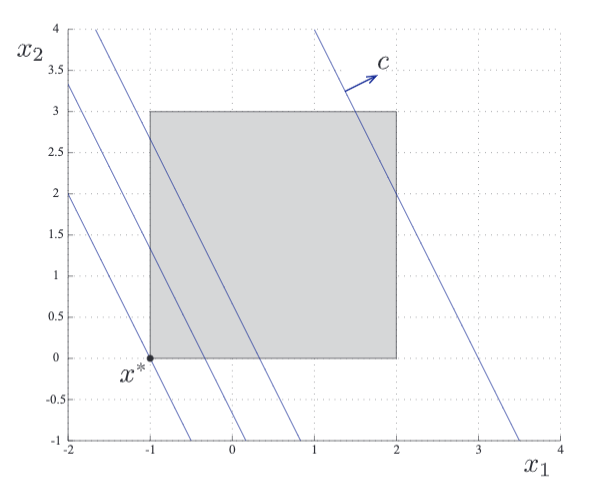
\includegraphics[scale=0.6]{toyLP.png}
    \caption{Visualization of the above LP, shamelessly borrowed from El Ghaoui's slides.}
\end{figure}

\begin{definition}[Polyhedral Functions]
    We say that a function $f:\RR^n\to \RR$ is \emph{polyhedral} if its epigraph is a polyhedron, that is if $\epi f = \{(x,t)\in \RR^{n+1}: f(x)\leq t\}$ can be represented as 
    \[ \epi f = \left\{ (x,t)\in \RR^{n+1}:\; C\colvec{2}{x}{t} \leq d\right\},\] 
    for some matrix $C\in \RR^{m,n+1}$ and vector $d\in \RR^m$. 
\end{definition}

Polyhedral functions include in particular functions that can be expressed as a maximum of a finite number of affine functions 
\[ f(x) = \max_{i=1,\dots, m} a_i^\T x + b_i,\] 
where $a_i \in \RR^n$, $b_i \in \RR$ for $i=1, \dots, m$. 
Indeed, the epigraph of such functions $f$ 
\[ \epi f = \{(x,t) \in \RR^{n+1}: \max_{i=1,\dots, m} a_i^\T x + b_i \leq t\}\] 
can indeed be expressed as the polyhedron 
\[ \epi f = \{(x,t) \in \RR^{n+1}: a_i^\T x + b_i \leq t, \; i = 1,\dots, m\}.\] 

Here are some more examples of polyhedral functions: 
\begin{itemize}
    \ii The $\ell_\infty$-norm function $f(x) = \|x\|_\infty$ is polyhedral since it can be written as the maximum of $2n$ affine functions 
    \[ f(x) = \max_{i=1\dots, n} \max(x_i, -x_i).\] 
    \ii The $\ell_1$-norm function $f(x) = \|x\|_1$ is polyhedral since it can be written as the sum of maxima of affine functions: 
    \[ f(x) = \sum_{i=1}^n \max(x_i, -x_i).\] 
    \ii Functions that are sums of maximums of affine functions (as discussed above) are polyhedral: 
    \[ f(x) = \sum_{j=1}^q \max_{i=1,\dots,m} a_{ij}^\T x + b_{ij}.\] 
    \ii Take $f$ as in the previous part again.
    The condition $(x,t)\in \epi f$ is equivalent to $\exists u\in \RR^q$ such that 
    \begin{align}
        \label{eq:epipoly}
        \sum_{j=1}^q u_j\leq t, \quad a_{ij}^\T x + b_{ij} \leq u_j, \; i = 1, \dots, m; \; j = 1,\dots, q.
    \end{align}
    The epigraph $\epi f$ is the projection (on the space of $(x,t)$-variables) of a polyhedron, so the epigraph itself is a polyhedron. 
   \end{itemize}

Polyhedral functions are convenient since minimizing them is equivalent to solving an LP. 
If $f$ is polyhedral, then 
\[ \min_x f(x)\quad \text{ s.t.: } Ax \leq b,\] 
can be written as 
\[ \min_{x,t} t\quad \text{ s.t.: } Ax\leq b, (x,t) \in \epi f.\] 

Since $\epi f$ is a polyhedron, we can express it as in Equation~\ref{eq:epipoly}, hence the problem above is an LP. 
However, note that the explicit representation of an LP in standard form may require the introduction of additional slack variables, which are needed for representation of the epigraph.

\subsection{Examples}
\begin{example}[$\ell_\infty$ regression problems]
    Take the following $\ell_\infty$ optimization problem: 
    \[ \min_x \|Ax - b\|_\infty, \quad A\in \RR^{m,n}, b\in \RR^{m}.\]
    The problem can first be rewritten in epigraphic form, adding a slack scalar variable $t$ 
    \[ \min_{x,t}\; t\quad \text{ s.t.: } \|Ax-b\|_\infty \leq t.\] 
    Then simply using the definition of the $\ell_\infty$ norm, observe that 
    \[ \|Ax-b\|_\infty \leq t \iff \max_{i=1,\dots,m} |a_i^\T x - b_i| \leq t \iff |a_i^\T x - b_i| \leq t, \; i = 1,\dots, m.\] 
    Hence, the problem is equivalent to the following LP in variables $x\in \RR^n$ and $t\in \RR$: 
    \begin{align*}
        \min_{x,t}\quad &t \\ 
        \text{ s.t. } &a_i^\T x - b_i \leq t, \quad i = 1,\dots, m \\ 
                                           &a_i^\T x - b_i \geq -t, \quad i = 1,\dots, m.
    \end{align*}
\end{example}

\begin{example}[$\ell_1$ regression problems]
    Here's another optimization problem using an $\ell_1$ norm instead:
    \[ \min_x \|Ax - b\|_1, \quad A\in \RR^{m,n}, b\in \RR^{m}.\]
    To convert this, we utilize a vector $u\in \RR^m$ of slack variables to get 
    \[ \min_{x,u} \sum_{i=1}^m u_i \quad \text{ s.t. } |a_i^\T x - b_i|\leq u_i,\; i=1,\dots, m.\] 
    This in turn is easily turned into a standard LP as follows:
    \begin{align*}
        \min_{x,u}\quad &\one^\T u \\
        \text{ s.t. } &a_i^\T x - b_i \leq u_i, \quad i = 1,\dots, m \\ 
                      &a_i^\T x - b_i \geq -u_i, \quad i = 1,\dots, m.
    \end{align*}
\end{example}

\newpage
\section{Thursday, February 25th: Convex Quadratic Programs}
\subsection{Convex Quadratic Functions and the QP Model}
A quadratic function in a vector of variables $x = \rowvec{4}{x_1}{x_2}{\cdots}{x_n}$ can be written generically as 
\[ f_0(x) = \frac 12 x^\T H x + c^\T x + d\] 
where $d\in \RR, c\in \RR^n$, and $H \in \RR^{n,n}$ is a symmetric matrix. 

This last condition can always be achieved, since if I had some arbitrary $n\times n$ matrix $A$ in my form, $x^\T A x = x^\T A^\T x$, so 
\[ x^\T A x = x^\T \left(\frac{A+A^\T}{2}\right) x,\] 
where the inside term is symmetric. 
So any quadratic form $x^\T H x$ can always be written as one where $H$ is symmetric; we refer to $H$ as the \emph{Hessian} of the quadratic function.

A quadratic function is said to be \emph{convex} if its Hessian is positive semi-definite, that is: every eigenvalue of the (symmetric) matrix $H$ is non-negative.
Convex quadratic functions typically look bowl-shaped, while non-convex ones can look saddle-like, etc. 

\begin{figure}[!htb]
    \centering
    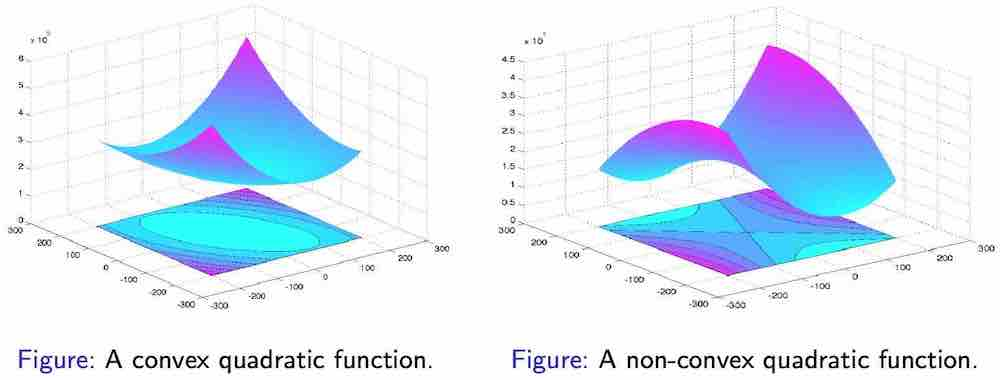
\includegraphics[scale=0.4]{qfconvex.jpeg}
    \caption{Taken from El Ghaoui's Slides.}
\end{figure}

\begin{definition}[Convex Quadratic Programs]
    Let $A\in \RR^{m,n}, b\in \RR^m$. The model 
    \begin{align*}
        \min \quad &f_0(x) \\ 
        \text{subject to: }\;\; & Ax\leq b, Cx = d,
    \end{align*}
    
    is called a \emph{quadratic program} (QP for short) if $f_0$ is a convex quadratic function, that is: 
    \[ f_0(x) = \frac 12 x^\T H x + c^\T x,\] 
    where $H = H^\T$ is positive semi-definite (PSD). 
\end{definition}
Note that $f_0$ is still quadratic if $H$ is not PSD, but the problem above would not be referred as a QP. 
An artifact of historical naming conventions, supposedly.

\subsubsection{Unconstrained QP Problems}

In the unconstrained setting, we can still employ our usual linear algebra techniques to minimize quadratic functions. 
Consider the convex quadratic function 
\[ p^* = \min_{x\in \RR^n} f(x) := \frac 12 x^\T H x + c^\T x + d.\] 

If $H\succ 0$ (PD), we can write 
\[ f(x) = \frac 12 (x-x_0)^\T H (x-x_0) + \alpha \geq \alpha,\] 
where $x_0 = -H^{-1}c, \alpha = d - \frac 12 x_0^\T H x_0$.
I think of this as completing the square, which you can see by expanding the above as 
\begin{align*}
    f(x) &= \frac 12 (x^\T H x - 2x_0^\T Hx + x_0^\T H x_0) + \alpha \\ 
         &= \frac 12 x^\T H x + (c^\T H^{-1}) H x + \frac 12 x_0^\T H x_0 + (d - \frac 12 x_0^\T H x_0)  \tag{since $H = H^\T$} \\ 
         &= \frac 12 x^\T H x + c^\T x + d 
\end{align*}

Then you know the quadratic form will always be greater than $0$ for nonzero $x-x_0$ by virtue of $H$ being positive-definite, so the best minimizer is to pick $x^* = x_0$.

If $H\succeq 0$ is only positive semi-definite, and $c\in \Rcal(H)$, then any $x_0$ such that $Hx_0 + c = 0$ is optimal by the same argument as before. 
Hencec, the set of solutions is given by 
\[ \{-H^\dagger c + \zeta,\; \zeta \in \Ncal(H)\}.\] 

Finally, if $H\succeq 0$ is PSD but $c\not\in \Rcal(H)$, then the function is unbounded below.
By the fundamental theorem, we can write $c$ as $c = -Hx_0 + r$, where $Hr = 0$ and for some $x_0, r\not= 0 \in \RR^n$.
Set $x(t) = x_0 - tr$ where $t\in \RR$, and note that 
\begin{align*}
    f(x(t)) &= \frac 12 (x_0-tr)^\T H (x_0 - tr) + (-Hx_0 + r)^\T (x_0 - tr) + d \\ 
            &= \frac 12 x_0^\T H x_0  - x_0^\T H x_0 + r^\T x_0 - t r^\T r \tag{since $Hr = 0$}  \\ 
            &= \text{constant} - t(r^\T r),
\end{align*}
which tends to $-\infty$ as $t \to\infty$, as we stated. 


\begin{example}[Least-Squares]
    Least-squares is actually a special case of an unconstrained QP model. 
    The problem ammounts to minimizing $f_0(x) = \|Ax-y\|_2^2$, where 
    \[ f_0(x) = (Ax-y)^\T (Ax-y) = x^\T A^\T A x - 2y^\T A x + y^\T y,\] 
    which is a quadratic function in standard form, with 
    \[ H = 2(A^\T A),\quad c = -2 A^\T y, \quad d = y^\T y.\] 
    Note that $f_0$ is convex since $A^\T A \succeq 0$. 
    Since this is unconstrained, and $c = -HA^\dagger y\in \Rcal(H)$, we have (from above) that the set of solutions is of the form 
    \[ \Xcal^{\text{opt}} = \{x^* = A^\dagger y + Nz : z\in \RR^r\},\] 
    wherer $r$ is the rank of $H$ (and column rank of $A$), and $N$ spans the nullspace of $A$. 

    If $A$ is full column rank, then $A^\T A \succ 0$, so the solution is unique and given by the well-known formula 
    \[ x^* = -H^{-1} c = (A^\T A)^{-1} A^\T y.\] 
\end{example}

\subsubsection{Linear Equality Constrained QP Problems}

If we have only linear equality constraints, then we can convert it into unconstrained form by eliminating the equality constraints (similar to how we did for linear systems).
Suppose we have the problem 
\begin{align*}
    \min \quad &f_0(x) := \frac 12 x^\T Hx + c^\T x + d\\ 
    \text{subject to: }\;\; & Ax\leq b,
\end{align*}
Parameterize all of the solutions $x$ to $Ax=b$ as $x = \bar{x} + Nz$, where $\bar{x}$ is a specific solution to $Ax=b$, $N$'s columns form a basis for $\Ncal(A)$, and $z$ is a vector of free variables.
Then we can substitute this in for $x$ in $f_0$ to get the unconstrained problem 
\[ \min_z \varphi_0(z) = \frac 12 z^\T \bar{H} z + \bar{c}^\T z + \bar{d},\] 
where 
\[ \bar{H} = N^\T H N,\; \bar{c} = N^\T (c + H\bar{x}),\; \bar{d} = d + c^\T \bar{x} + \frac 12 \bar{x}^T H \bar{x}.\] 

\subsection{Minimal cardinality solutions and \texorpdfstring{$\ell_1$}{l1}-norm problems}

Many engineering problems will concern themselves with finding solutions which are \emph{sparse}, i.e. contain few non-zero entries (low-cardinality solutions). 
This is a very natural requirement, since minimal representations tend to be the best explanations. 
However, finding minimum cardinality solutions (i.e. solutions with small $l_0$ norm) is hard in general, from a computational point of view. 
Thus, often several \emph{heuristics} are used in order to devise tractable numerical schemes which provide low cardinality solutions, such as using $\ell_1$ norm in place of the $\ell_0$ norm. 

For example, using the Cauchy-Schwartz inequality (Theorem~\ref{thm:cs}), we can obtain a close relation between $\card(x)$ and its $\ell_1$ norm. 
Let $\nz(x)$ be the vector whose $i$th entry is one whenever $x_i\not= 0$, and is zero otherwise, and $|x|$ is the vector of absolute values of all of the entries of $x$.
Note that $\|\nz(x)\|_2 = \card(x)$.
Then 
\[ \|x\|_1 = \nz(x)^\T |x| \leq \|\nz(x)\|_2 \cdot \|x\|_2 = \|x\|_2 \sqrt{\card(x)},\]
hence 
\[ \card(x) \leq k \implies \|x\|_1^2 \leq k \|x\|_2^2.\] 
Similarly, using Holder's (Theorem~\ref{thm:holder}) for $p = 1, q=\infty$, 
\[ \|x\|_1 = \nz(x)^\T |x| \leq \|\nz(x)\|_1 \|x\|_\infty = \|x\|_\infty\, \card(x),\] 
hence 
\[ \card(x) \leq k \implies \|x\|_1 \leq k\|x\|_\infty.\] 

The following example illustrates exactly how we can replace a cardinality constraint with one relying on the $\ell_1$ norm instead. 

\begin{example}[Piece-wise constant fitting]
    Suppose one observes a noisy time-series which is almost piece-wise constant. 
    The goal would be to find out what the constant levels are, which could correspond to states or levels of a system in applications. 

    Let $x\in \RR^n$ denote the signal vector (unknown), and $y\in \RR^n$ denote the vector of noisy signal observations (i.e. the true signal $x$ plus noise). 
    Given $y$, we want an estimate $\hat{x}$ of the original signal $x$ which has as few changes in consecutive time steps as possible. 
    This requirement can be modeled by minimizing the cardinality of the different vector $D\hat{x}$, where $D\in \RR^{n-1,n}$ is the difference matrix 
    \[ D = \bbm -1 & 1 & 0 & \dots & 0 \\ 0 & -1 & 1 & \dots & 0 \\  \vdots & & & \ddots &  \\ 0 & \dots & 0 & -1 & 1 \ebm,\] 
    so that $D\hat{x} = [\hat{x}_2-\hat{x}_1, \hat{x}_3-\hat{x}_2, \dots, \hat{x}_n - \hat{x}_{n-1}]^\T$. 

    Thus, we have the problem 
    \[ p^* = \min_{\hat{x}} f(\hat{x}) := \|y-\hat{x}\|_2^2\text{ s.t. } \card(D\hat{x}) \leq k, \] 
    where $k$ is an estimate on the number of jumps in the signal, and our objective function is measuring the error in our estimate. 

    We can get a \emph{lower bound} on the problem by noticing that we have the obvious solution $\hat{x} = 0$ which satisfies our cardinality constraint, and thus our optimal value must be lower than this. 
    Hence, $\|\hat{x}-y\|_2^2 \leq f(0) = \|y\|_2^2$ and so by triangle inequality, 
    \[ \|\hat{x}\|_2 = \|(\hat{x} - y) + y\|_2 \leq \|\hat{x}-y\|_2 + \|y\|_2 \leq 2\|y\|_2.\] 
Thus, using the cardinality results we obtained above, the constraint $\card(D\hat{x}) \leq k$ implies 
    \[ \|D\hat{x}\|_1 \leq \sqrt{k} \| D\hat{x}\|_2 \leq \sqrt{k} \|D\|_F \|x\|_2 \leq 2\sqrt{k}\|D\|_F\|y\|_2 =: \alpha.\]
    The relaxed problem is a QP of the form 
    \[ \min_{\hat{x}} \|y - \hat{x}\|_2^2 \quad \text{ s.t.: } \|D\hat{x}\|_1 \leq \alpha.\] 
    Alternatively, we could have instead chosen a problem with a weighted objective 
    \[ \min_{\hat{x}} \|y - \hat{x} \|_2^2 + \gamma \|D\hat{x}\|_1,\] 
    for some suitable parameter $\gamma \geq 0$. 
\end{example}

\begin{figure}[!htb]
    \centering
    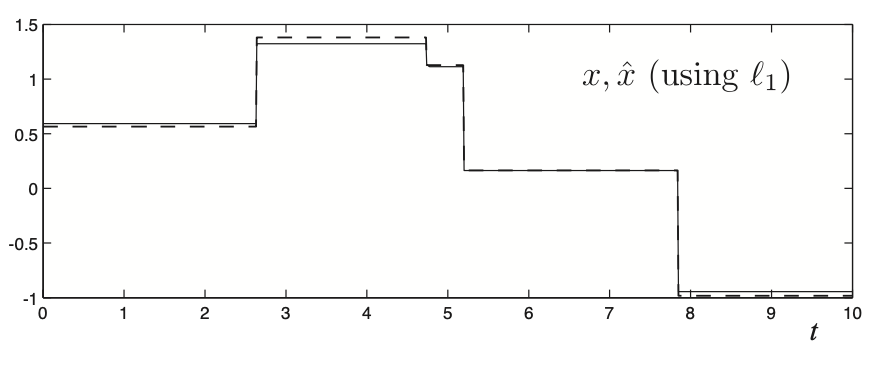
\includegraphics[scale=0.5]{pw_constant.png}
    \caption{Example of the piece-wise constant fitting problem and result achieved with $\ell_1$ objective. Taken from El Ghaoui's slides.}
\end{figure}

This general theme of using $\ell_1$ norms in our optimization problems leads to another important problem. 
Solving least-squares problems that, instead of having an $\ell_2$ regularization term as we've seen in the past, have an $\ell_1$ norm regularizer. 
\begin{example}[LASSO]
    Consider the following problem, known as the \emph{basis pursuit denoising problem} (BDPN), or as the \emph{least absolute shrinkage and selection operator} (LASSO) problem:
    \[ \min_{x\in \RR^n} \|Ax-y\|^2_2 + \la\|x\|_1, \quad \la \geq 0,\] 
    where $\|x\|_1 = |x_1|+\dots + |x_n|$.
    This problem has received much attention in recent years due to its relevance in the field of \emph{compressed sensing}. 

    The basic idea is that the $\ell_1$ norm is used as a proxy for the cardinality of $x$. 
    It formalizes a tradeoff between the accuracy with which $Ax$ approximates $y$, and the \emph{complexity} of the solution, i.e. the number of nonzero entries in $x$ (which can be interpreted as the number of relevant features, for example). 
    The larger $\la$ is, the more biased our problem is towards finding low-complexity solutions. 

    We can rewrite the above problem in standard QP form by introducing slack variables $u\in \RR^n$: 
    \begin{align*}
        \min_{x,u\in\RR^n}\quad &\|Ax-y\|_2^2 + \la \sum_{i=1}^n u_i \\ 
        \text{s.t. : }\;\; &|x_i|\leq u_i,\; i=1,\dots, n.
    \end{align*}
\end{example}

There are cool applications of LASSO to image compression in different bases, for example the wavelet basis, which is what modern JPEG compression schemes utilize. 
We also talked about Markowitz's mean-variance portfolio optimization model, which is central to modern portfolio theory. 

\newpage
\section{Tuesday, March 2nd: Second-Order Cone Models}
\subsection{Second-order cone programs}

Today, we'll be talking about \emph{second-order cone programming} (SOCP), which is a generalization of linear and quadratic programming which allows for affine combinations of variables to be constrained in a special convex set, called a \emph{second-order cone}. 
LPs and convex quadratic optimization fall under special cases of SOCP models, and they're quite useful in geometry problems, approximation problems, and probabilistic approaches to linear optimization. 

\begin{definition}[Second-Order Cone]
    The \emph{second-order cone} (SOC) in $\RR^3$ is the set of vectors $(x_1, x_2, t)$ such that $\sqrt{x_1^2+x_2^2} \leq t$ (i.e. the ice cream cone). 
    Horizontal sections of this set at level $\alpha \geq 0$ are discs of radius $\alpha$.

    In arbitrary dimensions, an $(n+1)$-dimensional SOC is the following set: 
    \[ \Kcal_n = \{(x,t), x\in \RR^n, t\in \RR : \|x\|_2 \leq t\}.\] 
\end{definition}

All of these cones point upwards however, so to capture the general notion of a second-order cone, we need to discuss what rotated second-order cones are. 
\begin{definition}[Rotated Second-Order Cone]
The rotated second-order cone in $\RR^{n+2}$ is defined by 
\[ \Kcal_n^r = \{(x,y,z), x\in \RR^n, y\in \RR^n,z\in \RR^n : x^\T x \leq 2yz, y\geq 0,z\geq 0\}.\] 
We can express this as a linear transformation (i.e. rotation) of our usual second order cones in $\RR^{n+2}$, since 
\[ \|x\|_2^2 \leq 2yz, y\geq 0, z\geq 0 \iff \left\|\colvec{2}{x}{\tfrac{1}{\sqrt{2}}(y-z)}\right\|_2 \leq \frac{1}{\sqrt{2}}(y+z),\] 
where the right hand side is a form in our original constraint from above.

\end{definition}
It's exactly as it sounds like: they're just second-order cones which are rotated, which is the purpose of the $y$ and $z$ parameters. 
Constraints of the form $\|x\|_2^2 \leq 2yz$ are usually referred to as \emph{hyperbolic constraints}. 
To see the equivalence between the two conditions, simply expand the $\ell_2$-norm condition as 
\[ \rowvec{2}{x}{\tfrac{1}{\sqrt{2}}(y-z)}\colvec{2}{x}{\tfrac{1}{\sqrt{2}}(y-z)} = x^\T x + \frac{1}{2} (y-z)^2 \leq \frac{1}{2}(y+z)^2 \iff x^\T x \leq 2yz\] 
as expected.


The standard format of a second-order cone constraint on a variable $x\in \RR^n$ expresses the condition that $(y,t) \in \Kcal_m$, with $y\in \RR^m, t\in \RR$ where $y,t$ are some affine functions of $x$. 
We can express these affine functions as $y = Ax+b$ and $t = c^\T x + d$, so the condition $(y,t) \in \Kcal_m$ becomes 
\begin{align}
\|Ax+b\|_2 \leq c^\T x + d,
\label{eq:soc}
\end{align}
where $A\in \RR^{m,n}, b\in \RR^m, c\in \RR^n,$ and $d\in \RR$. 

For example, our usual quadratic constraint 
\[ x^\T Qx + c^\T x \leq t, \quad Q\succeq 0\] 
can be expressed in conic form using the square root $Q^{1/2}$ (since $Q$ is PSD) as 
\begin{align}
\left\| \colvec{2}{\sqrt{2} Q^{1/2} x}{t-c^\T x - 1/2}\right\|_2 \leq t - c^\T x + 1/2.
\label{eq:quadsoc}
\end{align}

This can be achieved from our above transformation for rotated second-order cones, by writing our constraint as $\|\sqrt{2} Q^{1/2}x\|_2^2 \leq 2(t-c^\T x)$ and setting 
\[ \tilde{x} := \sqrt{2} Q^{1/2} x, \; \tilde{y} := \sqrt{2}(t-c^\T x),\; \tilde{z} := \tfrac{1}{\sqrt{2}}.\] 

Then 
\[ \frac{1}{\sqrt{2}}(\tilde{y}-\tilde{z}) = t - c^\T x - 1/2,\quad \frac{1}{\sqrt{2}}(\tilde{y}+\tilde{z}) = t - c^\T x + 1/2 \]
as we have seen.

Now we can define what an SOCP is.

\begin{definition}[Second-Order Cone Programs]
    A \emph{second-order cone program} is a convex optimization problem having \textbf{linear} objective and \textbf{SOC} constraints. 
    When the SOC constraints have the standard form in~(\ref{eq:soc}), we have a SOCP in \emph{standard inequality form} 
    \begin{align*}
        \min_{x\in \RR^n}& \quad c^\T x \\ 
        \text{s.t.:}& \quad \|A_i x + b_i \|_2 \leq c_i^\T x + d_i, \quad i = 1,\dots, m,
    \end{align*}
    where $A_i\in \RR^{m_i, n}$ are given matrices, $b_i\in \RR^{m_i}$, $c_i\in \RR^n$ are vectors, and $d_i$ are given scalars. 
\end{definition}

SOCPs are quite a large class of convex optimization problems; in fact, they generalize all of the convex optimization problems we've seen thus far, including LPs, convex QPs, and convex QCQPs. 

\subsection{Examples}
To demonstrate just how vast SOCPs really are, we'll show that basically every problem we've come across so far (and more!) can be written as an SOCP. 
\begin{example}[LPs are SOCPs]
    Any standard linear program in standard inequality form  
    \begin{align*}
        \min_{x\in \RR^n}& \quad c^\T x \\ 
        \text{s.t.:}& \quad a_i^\T x \leq b_i, \quad i = 1,\dots, m,
    \end{align*}
    can be easily written in SOCP form by setting the $\ell_2$-norm condition to zero and using just the affine part, as 
    \begin{align*}
        \min_{x\in \RR^n}& \quad c^\T x \\ 
        \text{s.t.:}& \quad \|C_i x + d_i \|_2 \leq b_i - a_i^\T x, \quad i = 1,\dots, m,
    \end{align*}
    where $C_i = 0, d_i = 0$ for $i = 1, \dots, m$. 
\end{example}

\begin{example}[QPs are SOCPs]
    Any standard quadratic program in standard form  
    \begin{align*}
        \min_{x\in \RR^n}& \quad x^\T Q x + c^\T x \\ 
        \text{s.t.:}& \quad a_i^\T x \leq b_i, \quad i = 1,\dots, m,
    \end{align*}
    where $Q = Q^\T \succeq 0$ can be written in SOCP form as 
    \begin{align*}
        \min_{x,y}& \quad c^\T x +y \\ 
        \text{s.t.:}& \quad \left\|\colvec{2}{2Q^{1/2} x}{y-1}\right\|_2 \leq y+1, \\ 
                    & \quad a_i^\T x \leq b_i, \quad i = 1, \dots, m.
    \end{align*}
    The trick is to convert the quadratic form constraint into an inequality.
    First, we set $y = x^\T Q x$. 
    Then use our earlier form for quadratic constraints~(\ref{eq:quadsoc}) to write $x^\T Q x \leq y$ in the form presented here by setting $c^\T x = 0$ and adjusting constants.
    
    Directly expanding the constraint here gives us 
    \[ 4x^\T Q x + (y-1)^2 \leq (y+1)^2 \iff x^\T Q x\leq y,\] 
    which corresponds to our quadratic form condition. 
\end{example}

\begin{example}[QCQPs are SOCPs]
    Any convex quadratic-constrained quadratic programs of the form
    \begin{align*}
        \min_{x\in \RR^n}& \quad x^\T Q_0 x + a_0^\T x \\ 
        \text{s.t.:}& \quad x^\T Q_i x + a_i^\T x \leq b_i, \quad i = 1,\dots, m,
    \end{align*}
    where $Q_i = Q_i^\T \succeq 0$ can be written in SOCP form as 
    \begin{align*}
        \min_{x,t}& \quad a_0^\T x +t \\ 
        \text{s.t.:}& \quad \left\|\colvec{2}{2Q_0^{1/2} x}{t-1}\right\|_2 \leq t+1, \\ 
                    & \quad \left\|\colvec{2}{2Q_i^{1/2} x}{b_i-a_i^\T x - 1}\right\|_2 \leq b_i - a_i^\T x + 1, \; i = 1, \dots, m
    \end{align*}
    using the same idea as before.
\end{example}

For a new example, consider the problem of sums of norms, i.e. 
\[ \min_x \sum_{i=1}^p \|A_i x - b_i\|_2,\] 
where $A_i \in \RR^{m,n}, b_i\in \RR^m$ are given data.
This can be easily written as an SOCP by introducing auxiliary scalar variables $y_1, \dots, y_p$ to make our objective linear, so 
\begin{align*}
    \min_{x,y}& \quad \sum_{i=1}^p y_i \\ 
    \text{s.t.:}& \quad \|A_i x - b_i \|_2 \leq y_i, \quad i = 1,\dots, p
\end{align*}

Similarly, the maxima of norms problem 
\[ \min_x \max_{i=1,\dots,p} \|A_i x - b_i\|_2,\] 
can be cast in SOCP form as 
\begin{align*}
    \min_{x,y}& \quad y \\ 
    \text{s.t.:}& \quad \|A_i x - b_i \|_2 \leq y, \quad i = 1,\dots, p
\end{align*}

It's important to note that while the constraint $\|z\|_2 \leq y$ is convex and can be optimized over, $\|z\|_2^2 \leq y^2, y\geq 0$ is \emph{not convex}, so we can't optimize over it.

\begin{example}[Square-root LASSO]
    Consider the optimization problem 
    \[ p^* := \min_w \|X^\T w - y\|_2 + \la \|w\|_1\] 
    where $X$ is our data matrix, with $\la > 0$ a sparsity-inducing parameter. 
    This is square-root LASSO, as we're missing the usual squared term on the $\ell_2$-norm for our loss. 

    This turns out to be an SOCP as well, of the form 
    \[ \min_{w,v,t} t + \la \sum v_i \quad \text{ s.t.: } t \geq \|X^\T w - y\|_2,\; v_i \geq w_i \geq -v_i \;\forall i.\] 
\end{example}


\begin{example}[Examplar Selection]
    In examplar selection, we are given a data matrix $X = [x_1,\dots, x_m]\in \RR^{m,n}$, where columns $x_i$ are the data points. 
    We wish to find a small subset of data points which are approximately representative of the whole dataset. 
    Precisely, we seek to find a sparse subset of data points $\{x_j\}_{j\in \Jcal}$, with $\Jcal\subseteq \{1,\dots, m\}$ some indexing set, such that 
    \[ \forall i\in \{1, \dots, n\}, \; x_i \approx \sum_{j\in \Jcal} x_j w_{ij}.\] 
    In other words, every data point can be accurately represented as a linear combination of the same few data points. 
    We can write the above condition as $X \approx XW^\T$, where $W$ has a lot of its columns entirely zero. 

    We can model this as an SOCP: 
    \[ \min_{W = [w_1, \dots, w_m]} \|X - XW^\T \|_F : \quad \sum_{j=1}^m \|w_j\|_2 \leq \kappa,\] 
    where a small value of parameter $\kappa > 0$ encourages many columns in $W$ to be entirely zero. 

    Note that the constraint here is essentially an $\ell_1$-norm on the $w_i$ column norms, so we're doing a LASSO-like feature selection to find the sparse set $\Jcal$. 
    Also, we can easily write the Frobenius norm as a sum of $\ell_2$ constraints on the column norms of the inside matrix.
    So this is indeed an SOCP.
\end{example}

Finally, SOCP can also model problems involving powers of variables. 
For example, consider the following variant of least-squares: 
\[ p^* := \min_w \|X^\T w - y\|_2 + \la \sum_{i=1}^n |w_i|^\alpha, \] 
where $\alpha > 1$ is the ratio of two integers. 
Notice that $\alpha = 1$ gives us LASSO, while $\alpha = 2$ gives us Ridge regression. 
A typical choice is $\alpha \in (1,2)$ to achieve a good trade-off between encouraging sparsity and robustness to noise. 

For example, take $\alpha = 3/2$. 
The condition $t \geq u^{3/2}$ for $u \geq 0$ is equivalent to the existence of $v\geq 0$ such that 
\[ vt \geq u^2, u \geq v^2.\] 
Hence we can rewrite this as an SOCP with rotated cone constraints 
\[ p^* = \min_{w,v,u,t} \|X^\T w - y\|_2 + \la \sum_{i=1}^n t_i : \quad t\geq 0, u\geq |w|,\] 
\[ v_i t_i\geq u_i^2, u_i \geq v_i^2, i = 1,\dots, n.\] 

We ended on an interesting discussion of PCA vs LASSO, i.e. how are they different in dimensionality reduction and sparsity. 
The summary is that PCA gives you the directions of most variance (in an unsupervised manner), but provides no sparsity nor interpretability of the resulting data. 
LASSO provides intepretability and sparsity, but requires labels in order to do so (and hence is supervised). 

There is something called sparse PCA which can give you directions with sparser projections though, which could be considered somewhere in between the two.

\newpage
\section{Thursday, March 4th: Robust Optimization Models}

\subsection{Robust optimization framework}
Consider a ``nominal'' optimization problem (meaning the original, idealistic no-noise model) 
\[ \min_x f_0(x) \; : \; f_i(x) \leq 0, i = 1,\dots, m.\] 
In practice, our problem data is \emph{uncertain}, i.e. 
\begin{itemize}
    \ii \emph{Estimation} errors affect problem parameters
    \ii \emph{Implementation} errors affect the decision taken.
\end{itemize}

Uncertainties often lead to highly unstable solutions or much degraded realized performance. 
These problems are even compounded in problems with multiple decision periods! 

We call this the \emph{curse of uncertainty}, and the goal of today's lecture is to formalize a framework for fixing nominal problems to be more robust.

Consider the nominal optimization problem from above
\[ \min_x f_0(x) \; :\; f_i(x) \leq 0, i=1,\dots, m.\] 
It is possible now that each of these values in our functions is uncertain and has unknown parts. 
For example, if $f_0(x)$ is modeled as $c^\T x$ where $c$ is known, it's possible that there is an unknown $u$ (noise or uncertainty) for which our function is actually $f_0(x,u) = (c+u)^\T x$, for $\|u\|_\infty \leq .01$. 

Our functions $f_i$ then depend on a second variable $u$, the ``uncertainty'', which is constrained to lie in a given set $\Ucal$. 
This creates the \emph{robust counterpart} to our optimization problem:
\[ \min_x\; \max_{u\in \Ucal} f_0(x,u) \; : \; \forall u\in \Ucal,\; f_i(x,u) \leq 0, i = 1,\dots, m.\] 

You could think of this as playing a game, where the uncertainty is trying to make your life as hard as possible, and you need to minimize your objective in light of that. 

This inherits convexity from the nominal, and is very tractable in some practically relevant cases. 
In general though, the robust counterpart has high complexity, but there are systematic ways to get relaxations. 

You could also consider other cost functions instead of a $\max$ over all $u$'s (which is a worst-case estimate); other options are to integrate over all values of $f_0$, or averaging. 

Let's look at robustifying linear programs in particular. 
Take the nominal problem 
\begin{align}
\text{(nominal) }\min_x c^\T x : a_i^\T x \leq b_i, i = 1, \dots, m.
\label{eq:nomLP}
\end{align}

Assume for now that $a_i$ is only known to belong to a given set $\Ucal_i \subseteq \RR^n$ (we will soon generalize to errors everywhere). 
For example, we could have $a_i \in \Ucal_i = \{\hat{a}_i + u_i : \|u_i\|_\infty \leq \eps\}.$
Then our robust counterpart to~(\ref{eq:nomLP}) would be 

\[ \text{(robust) }\min_x c^\T x : \forall a_i\in \Ucal_i, a_i^\T x \leq b_i, i = 1,\dots, m.\] 

If we assume instead that the cost vector $c$ in~(\ref{eq:nomLP}) is only known to belong to a given set $\Ucal \subseteq \RR^n$, then our robust counterpart would be 
\[ \text{(robust) }\min_x \max_{c\in\Ucal} c^\T x : a_i^\T x \leq b_i, i = 1,\dots, m.\] 

In general we can extend this robust approach to uncertainties affecting the cost vectors, coefficient matrix, and the right-hand side vector $b$. 
The solution may be hard, but it becomes easy for special uncertainty sets, which we'll examine now. 

\subsection{Special Uncertainty Sets for Robust LPs}
Let's examine the robust counterpart to a single inequality constraint 
\[ \forall a\in \Ucal,\; a^\T x \leq b\]
where $\Ucal$ takes the following forms: 
\begin{itemize}
    \ii scenario uncertainty: $\Ucal$ is a finite set ``scenarios''; 
    \ii $\Ucal$ is a box.
    \ii $\Ucal$ is a sphere, or more generally an ellipsoid; 
\end{itemize}

The above constraint can be written as 
\[ b \geq \max_{a\in \Ucal} a^\T x.\] 

\begin{itemize}
    \ii \textbf{Scenario uncertainty}: This model assumes that the coefficient vector $a$ is only known to lie in a finite sets in $\RR^n$, say 
    \[ \Ucal = \{a^{(1)}, \dots, a^{(K)}\}\]
    with $a^{(k)}$ a ``scenario'', $k = 1,\dots, K$. 
    We then have 
    \[ \max_{a\in \Ucal} a^\T x = \max_{1\leq k \leq K} (a^{(k)})^\T x \leq b.\] 
    For example, when $\Ucal$ is a finite set of three scenarios, our feasible set $\{x: a^\T x \leq b,\; \forall a\in \Ucal\}$ will be a polyhedron made up of three half-spaces. 
\end{itemize}

\begin{minipage}{0.5\textwidth}%
    \centering
    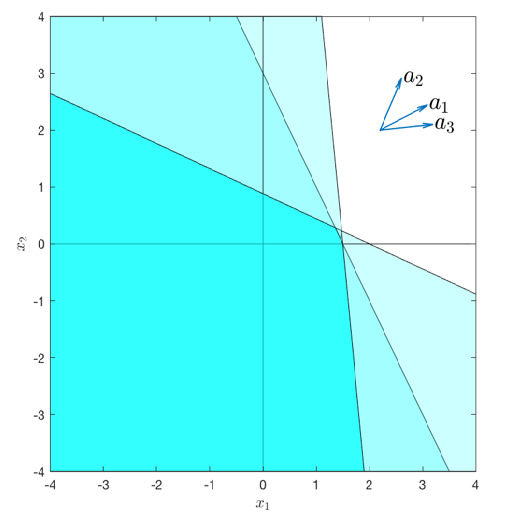
\includegraphics[scale=0.7]{scenario_uncertainty.png}
    \captionof{figure}{Scenario uncertainty.}
\end{minipage}%
\begin{minipage}{0.47\textwidth}
    \centering
    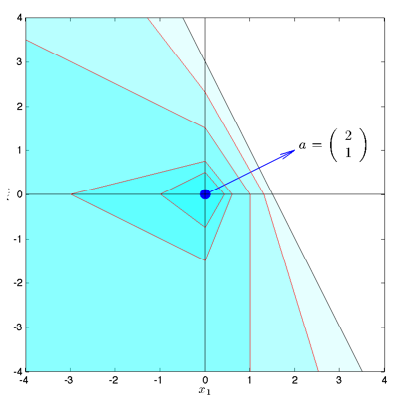
\includegraphics[scale=0.87]{box_uncertainty.png}
    \captionof{figure}{Box uncertainty for $\rho=0,0.1,$ $0.2,\dots$. The straight line is $\rho=0$.}
\end{minipage}

\begin{itemize}
    \ii \textbf{Box uncertainty}: This model assumes that the coefficient vector $a_i$ is only known to lie in a ``box'' (or hyper-rectangle in $\RR^n$). 
    In its simplest case, this uncertainty model has the form 
    \[ \Ucal = \{a : \|a-\hat{a}\|_\infty \leq \rho\} = \{a + \rho u : \|u\|_\infty \leq 1\},\] 
    where $\rho \geq 0$ is a measure of the size of the uncertainty, and $\hat{a}$ is the nominal value of the coefficient vector. 
    We have 
    \[ \max_{a\in \Ucal} a^\T x = \hat{a}^\T x + \rho\cdot \left(\max_{u:\|u\|_\infty \leq 1} u^\T x\right) = \hat{a}^\T x + \rho\|x\|_1 \leq b.\] 
    When $\Ucal$ is a box, the set $\{x:a^\T x \leq b, \; \forall a\in\Ucal\}$ is a polyhedron with at most $2^n$ vertices.
    For big enough $\rho$, some of the $a$'s will have different signs when taking inner products ($a^\T x$). 
    The hyperplanes will then face opposite and enclose a space, leading to the box shape we see above.

    \ii \textbf{Spherical uncertainty}: This model has similar assumptions to the box uncertainty, except that the coefficient vector $a_i$ is only known to lie in a sphere, i.e. 
    \[ \Ucal = \{a : \|a-\hat{a}\|_2 \leq \rho\} = \{a + \rho u : \|u\|_2 \leq 1\},\] 
    where $\rho \geq 0$ is a measure of the size of the uncertainty, and $\hat{a}$ is the nominal value of the coefficient vector. 
    We have 
    \[ \max_{a\in \Ucal} a^\T x = \hat{a}^\T x + \rho\cdot \left(\max_{u:\|u\|_2 \leq 1} u^\T x\right) = \hat{a}^\T x + \rho\|x\|_2 \leq b\] 
    by Cauchy-Schwarz (Theorem~\ref{thm:cs}). 

    Notice that this condition is an SOCP constraint, which alludes to why they're so well studied currently. 
    So when $\Ucal$ is a sphere, the feasible set is defined by a single SOCP constraint. 

    \begin{figure}[!htb]
        \centering
        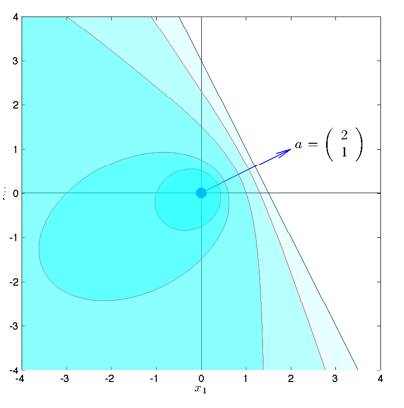
\includegraphics[scale=0.7]{spherical_uncertainty.png}
        \caption{Spherical uncertainty.}
    \end{figure}

    \ii \textbf{Ellipsoidal uncertainty}: The uncertainty set in this model has form 
    \[ \Ucal = \{a : (a-\hat{a})^\T P^{-1} (a-\hat{a}) \leq 1\}, \] 
    where $\hat{a}$ is the nominal coeffficient vector as usual, and $P = P^\T \succ 0$ determines the shape and size of the ellipse. 
    Since $P\succ 0$, we can write $P = R^\T R$ for some matrix $R$ and get 
    \[ \Ucal = \{a = \hat{a} + Ru : \|u\|_2 \leq 1\},\] 
    as $u = R^{-1}(a-\hat{a})$ gives back our original condition. 
    So 
    \[ \max_{a\in \Ucal} a^\T x = \hat{a}^\T x + \max_{u: \|u\|_2 \leq 1} (Ru)^\T x = \hat{a}^\T x + \|R^\T x \|_2 \leq b,\] 
    which is again an SOC constraint.
\end{itemize}

Next we can discuss what robust LP looks like with each of these uncertainty constraints, and look at the geometry of the feasible sets. 

The robust LP with box uncertainty 
\begin{align*}
    \min_x\; c^\T x \quad\text{ s.t.: } \forall a_i\in \Bcal_i,\; a_i^\T x \leq b_i \quad i = 1,\dots, m,
\end{align*}
where $\Bcal_i = \{\hat{a}_i + \rho_i u : \|u\|_\infty \leq 1\}$ is 
\begin{align*}
    \min_x\; c^\T x \quad\text{ s.t.: } \hat{a}_i^\T x + \rho_i\|x\|_1 \leq b_i \quad i = 1,\dots, m.
\end{align*}

This can be expressed in standard LP form with our usual tricks as 
\begin{align*}
    \min_x\; c^\T x \quad\text{ s.t.: } &\hat{a}_i^\T x + \rho_i\sum_{j=1}^n u_j \leq b_i \quad i = 1,\dots, m, \\
                                        & -u_j \leq x_j \leq u_j, \quad j = 1, \dots, n.
\end{align*}

Looking at the geometry, we see that the robust counterpart's feasible set is inside the nominal feasible set, and has polyhedral boundaries; it's still an LP! 

\begin{minipage}{0.5\textwidth}%
    \centering
    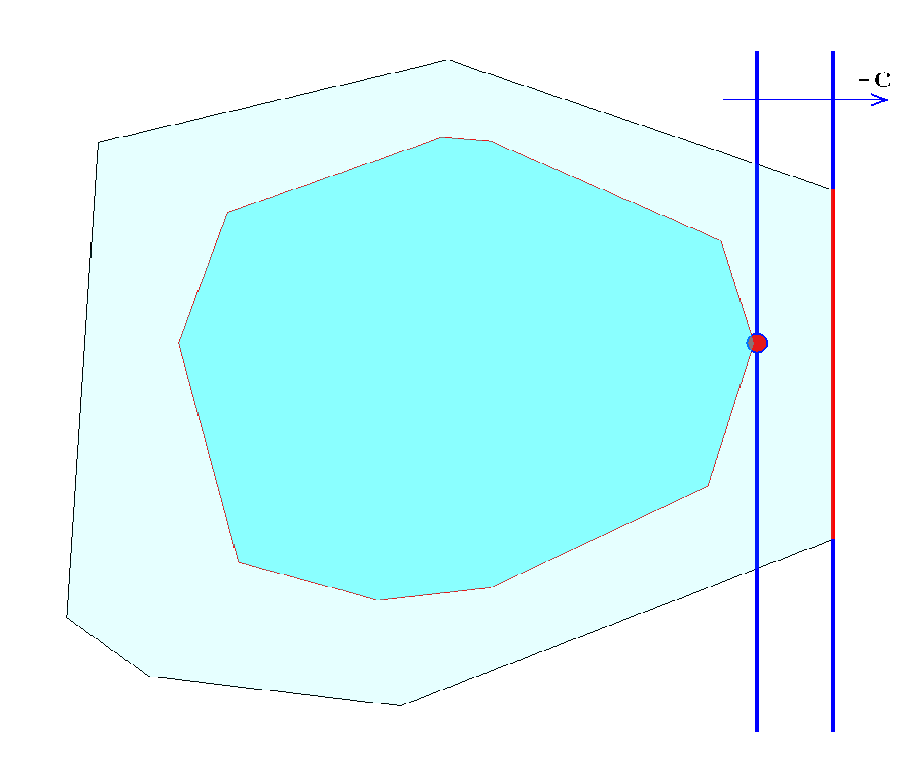
\includegraphics[scale=0.45]{robust_lp_box.png}
    \captionof{figure}{Robust LP with box uncertainty.}
\end{minipage}%
\begin{minipage}{0.47\textwidth}
    \centering
    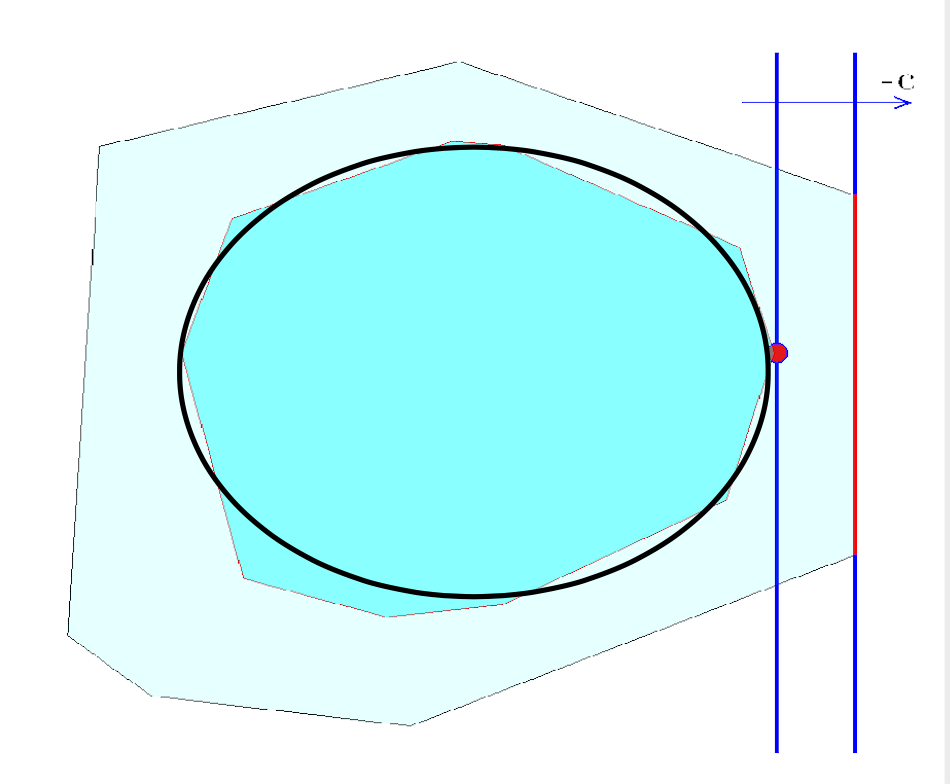
\includegraphics[scale=0.45]{robust_lp_spherical.png}
    \captionof{figure}{Robust LP with spherical uncertainty (feat. my Paint skills).}
\end{minipage}
\vspace{0.2cm}

On the other hand, with spherical uncertainty, the robust counterpart's feasible set is also inside the nominal feasible set, but its boundaries are smooth, making the solution unique. 
This makes the robust solution less sensitive to data changes, while the nominal LP has many optimal point (red line), which means solutions may be very sensitive. 

\subsection{Chance-constrained LP}
Chance constrained linear programs arise naturally from standard LPs when some of the data could be uncertain and random. 
Then we want to model some of our variables as random variables, which generally would make the problem too hard to solve, but under certain assumptions we can arrive at some results.

As always, consider the standard inequality form LP 
\[ \min_x\; c^\T x \quad \text{s.t.: } a_i^\T x \leq b_i, \; i = 1,\dots, m.\] 
Suppose that the problem data vectors $a_i$ are not knonw precisely, but rather are random vectors modeled by multivariate Gaussians with mean value $\EE\{a_i\} = \bar{a}_i$ and covariance matrix $\var\{a_i\} = \Sigma_i \succ 0$. 
In this case, the scalar $a_i^\T x$ is also a random variable, specifically a normal random variable with 
\[ \EE\{a_i^\T x\} = \bar{a}_i^\T x, \quad \var\{a_i^\T x\} = x^\T \Sigma_i x.\] 

However, this means it makes no sense to impose a constraint of the form $a_i^\T x\leq b_i$, since the LHS is a normal random variable and can assume any value. 
So this constraint can always be violated by some outcomes of our random data $a_i$. 
Instead, we only ask for this constraint to be satisfied up to a given level of probability $p_i \in (0,1)$ chosen \emph{a priori} by the user. 
This represents the probabilistic \emph{reliability} at which the constraint will be satisfied despite random fluctuations in data. 

In summary, we can define chance-constrained LPs as follows: 
\begin{definition}[Chance-constrained LPs]
    The \emph{chance-constrained} (or probability constrained) counterpart of the standard nominal LP is 
    \begin{align}
    \min_x\; c^\T x \quad\text{ s.t.: } \Pr\{a_i^\T x \leq b_i\} \geq p_i, \quad i = 1,\dots, m,
    \label{eq:chanceLP}
    \end{align}
where $p_i$ are the assigned reliability levels. 
\end{definition}

We have the following result that demonstrates this chance-constrained LP can be modeled by an SOCP. 

\begin{theorem}[Chance-constrained LPs are SOCP]
    Consider the problem in~(\ref{eq:chanceLP}), under the assumptions that $p_i > 0.5$ for $i = 1,\dots, m$, and that $a_i$ are independent, normal random vectors with means $\bar{a}_i$ and covariance matrices $\Sigma_i \succ 0$. 
    Then the chance-constrained LP presented in~(\ref{eq:chanceLP}) is equivalent to the SOCP 
    \begin{align*}
        \min_x\; c^\T x\quad \text{ s.t.: } \bar{a}_i^\T x \leq b_i - \Phi^{-1}(p_i) \|\Sigma_i^{1/2} x\|_2,\quad i = 1,\dots, m,
    \end{align*}
    where $\Phi^{-1}(p)$ is the inverse cumulative probability distribution of a standard normal variable.
\end{theorem}

Notice that this constraint can be rewritten as 
\[ \bar{a}_i^\T x + \kappa_i \sqrt{x^\T \Sigma_i x} \leq b_i,\] 
where $\kappa_i = \Phi^{-1}(p_i)$ represents the $z$-score of the reliability level $p_i$, and $\sqrt{x^\T \Sigma_i x}$ represents the standard deviation of $\bar{a}^\T x$. 
This last term can be thought of as regularization.

\subsection{Robust Least-Squares}
Suppose we start with our standard LS problem 
\[ \min_x \|Ax - y\|_2, \quad A\in \RR^{m,n},\; y\in\RR^m.\]
Now assume that $A$ is only known to be within a certain ``distance'' to a given ``nominal'' matrix $\hat{A}$ (as we have throughout this lecture). 
Mathematically, we will formulate that 
\[ \|A - \hat{A} \|_2 \leq \rho,\] 
where $\|\cdot\|_2$ denotes the $\ell_2$ operator norm (which coincides with the largest singular value norm, see Sec~\ref{subsec:svd_norms}), 
and $\rho\geq 0$ measures the size of the uncertainty.
Equivalently, $A = \hat{A} + \Delta$ where $\Delta$ is the uncertainty, and $\|\Delta\|_2 \leq \rho$. 

The \emph{robust least-squares} problem is then the following: 
\[ \min_x \max_{\|\Delta \|_2 \leq \rho} \| (\hat{A} + \Delta)x - y \|_2.\] 

We want to minimize (over $x$) our worst-case value of our residual error under the uncertainty of $\Delta$. 

The solution is quite simple. 
We can solve the inner maximization, first by using the convexity (or just the triangle inequality) of the Euclidean norm to get 
\[ \|(\hat{A} + \Delta)x - y \|_2 \leq \|\hat{A}x - y\|_2 + \|\Delta x\|_2.\] 

By properties of the operator norm, we can simplify this last term as 
\[ \|\Delta x\|_2 \leq \|\Delta\| \cdot \|x\|_2 \leq \rho \|x\|_2.\] 
Thus we obtain a bound on the objective value of our robust LS problem: 
\[ \max_{\|\Delta \|_2 \leq \rho} \| (\hat{A} + \Delta)x - y \|_2 \leq \|\hat{A}x-y\|_2 + \rho \|x\|_2.\] 
This is actually achieved for some choice of $\Delta$, so our original robust LS problem is equivalent to  
\[ \min_x \|\hat{A} x - y\|_2 + \rho\|x\|_2,\] 
i.e. our nominal problem with some regularization penalty. 
This, in turn, can be easily cast into SOCP form as 
\[ \min_{x,u,v}\quad u + \rho v \quad \text{s.t. } u\geq \|\hat{A}x -y\|_2,\; v \geq \|x\|_2.\] 

\section{Tuesday, March 9th: Review}
We just did review. 

\section{Thursday, March 11th: Midterm 1}
We had our midterm. 

\newpage
\section{Tuesday, March 16th: Convexity}
Today, we will be talking about the key feature that makes an optimization problem ``nice'', which is a property called \emph{convexity}. 
In this lecture, we characterize convex sets and convex functions. 
In the next, we'll define convex optimization problems as those where a convex objective function is minimized over a convex set. 
This will be useful, as certain types of convex models will have special tech which makes solving and modeling them much easier. 

\subsection{Convex Sets}

\subsection{Convex Functions}

One operation that preserves convexity is an affine variable transformation. 
Let $f:\RR^n\to\RR$ be convex, and define 
\[ g(x) = f(Ax+b), \quad A \in \RR^{n,m}, b\in \RR^n.\] 
Then $g$ is convex over $\dom g = \{x : Ax + b \in \dom f\}$. 
\begin{example}[Examples of Affine Convex Operations]
    We have $f(z) =  -\log (z)$ is convex over $\dom f = \RR_{>0}$, so $f(x) = -\log(ax+b)$ is also convex over $ax+b>0$. 

    Another common example is the use of convex loss functions in machine learning. 
    For any convex function $\Lcal :\RR\to\RR$, the function 
    \[ (w,b) \in \RR^n \times \RR \to \sum_{i=1}^m \Lcal(w^\T x_i + b),\] 
    where $x_1, \dots, x_m\in\RR^n$ are given data points, is convex. 
    For example, one common case would be the least squares loss $\Lcal(z) = \|z-y\|_2^2$. 
\end{example}

If $(f_\alpha)_{\alpha\in\Acal}$ is a family of convex functions, then the pointwise max function 
\[ f(x) = \max_{\alpha\in\Acal} f_\alpha (x)\] 
is convex over the domain $\{\cap_{\alpha\in \Acal} \dom f_\alpha\} \cap \{x : f(x) < \infty\}.$

\subsection{Characterizations of Convexity}


\newpage
\section{Thursday, March 18th: Convex Optimization Problems}
\subsection{Nomenclature}
\subsection{Examples}
\subsection{Problem transformations}

\newpage
\section{Tuesday, March 30th: Weak Duality}

\subsection{Weak duality}
Consider an optimization problem in standard form 
\begin{align*}
    p^* = \min_{x\in\RR^n} \quad & f_0(x) \\ 
    \text{subject to: } \quad & f_i(x) \leq 0, \quad i = 1,\dots, m, \\ 
                              & h_i(x) = 0, \quad i = 1,\dots, q,
\end{align*}
and let $\Dcal$ denote the domain of this problem, assumed to be nonempty. 

We refer to the above problem as the \emph{primal} problem. 
Note we are not assuming the convexity of $f_i, h_i$ currently. 

\begin{example}
    Illustrative example.
\end{example}

We have the following definition: 
\begin{definition}[Lagrangian]
    The \emph{Lagrangian} of a primal optimization problem is the function 
    \[ \Lcal(x,\la,\nu) = f_0(x) + \sum_{i=1}^m \la_i f_i(x) + \sum_{i=1}^q \nu_i h_i(x)\] 
    where $x\in \RR^n$, $\la \in \RR^m$, and $\nu\in \RR^q$. 
    The vectors $\la$ and $\nu$ are referred to as \emph{Lagrange multipliers}, or dual variables.
\end{definition}

Using the Lagrangian, we can express our problem in min-max form as 
\[ p^* = \min_x \max_{\la\geq 0, \nu} \Lcal(x,\la,\nu).\] 
This is due to the fact that for any $x$, 
\[ \max_{\la\geq 0, \nu} \Lcal(x,\la,\nu) = \begin{cases} f_0(x) \quad \text{ if } x\text{ is feasible,} \\ +\infty \quad \text{otherwise}.\end{cases}.\] 
We've seen this technique before, where we can remove the constraints in the problem by defining ourr objective to be $+\infty$ outside of our feasible set. 

We have the following relationship between $\min\max$ and $\max\min$: 
\begin{theorem}[Minimax inequality]
For any sets $X,Y$ and any function $F: X\times Y\to \RR$, 
\[ \min_{x\in X} \max_{y\in Y} F(x,y) \geq \max_{y\in Y} \min_{x\in X} F(x,y).\] 
\end{theorem}
\begin{proof}
    For any $(x_0, y_0) \in X\times Y$, the value of $F(x_0, y_0)$ has to wedge itself between the $\min_{x\in X}$ and the $\max_{y\in Y}$. 
    In equations, 
    \[ h(y_0) := \min_{x\in X} F(x,y_0) \leq F(x_0, y_0) \leq \max_{y\in Y} F(x_0, y) =: g(x_0),\]
    so $h(y_0) \leq g(x_0)$.
    Since this was for any $(x_0, y_0)$, we can take $y_0$ to be the max over $Y$ and $x_0$ to be the min over $X$.
\end{proof}

We can illustrate this point in the interpretation of a game, in which case it's always better to go first (if first is the maximizing player). 

Applying the minimax inequality to the Lagrangian, we obtain 
\[ p^*  = \min_x \max_{\la\geq 0, \nu} \Lcal(x,\la, \nu) \geq \max_{\la\geq 0,\nu} \min_x \Lcal(x,\la,\nu) =: d^*.\] 
The problem on the right is called the \emph{dual problem}, and it involves maximizing (over $\la\geq 0, \nu$) the \emph{dual function} 
\begin{align*}
    g(\la,\nu) &:= \min_x  \Lcal(x,\la,\nu) \\ 
               &= \min_x f_0(x) + \sum_{i=1}^m \la_i f_i(x) + \sum_{i=1}^q \nu_i h_i(x).
\end{align*}
This function is the pointwise minimum of affine (and therefore concave) functions in $(\la, \nu)$, so $g$ itself is concave. 
Hence the dual problem, a concave maximization problem over a convex set $(\RR^m_+ \times \RR)$, is convex!

<probability simplex projection duality>

In fact, strong duality does hold sometimes, i.e. $p^* = d^*$, specifically for projection on the probability simplex.
For every $\nu\in \RR$, the solution to the problem 
\[ \min_{x\geq 0} \Lcal(x,\nu)\] 
is unique, and characterized by the zero-gradient condition $\nabla_x \Lcal(x,\nu) = 0$, leading to 
\[ x_i^*(\nu) = \max(0, z_i + \nu), \quad i = 1,\dots, m.\] 
In addition, the dual function $g$ is smooth, and at its maximum its gradient is zero: 
\[ 0 = \nabla_\nu g(\nu^*) = 1 - \sum_{i=1}^n \max(0, z_i + \nu^*) = 1 - \sum_{i=1}^n x_i^* (v^*),\] 
which proves that the point $x^* (v^*)$ is feasible for the primal problem. 

\begin{example}[Sum of $k$ largest elements]
For given $w\in \RR^n$ and $k\in \{1,\dots, n-1\}$, define 
\[ s_k(w) = \sum_{i=1}^k w_{[i]},\] 
where $w_{[i]}$ is the $i$-th largest element in $w$.

The function $s_k$ is convex, since $s_k$ is just a maximum of all $k$-wise sums of $w_i$'s, and hence pointwise maximums holds. 
\begin{align*}
    s_k(w) &= \max_{\Ical} \sum_{i\in\Ical} w_i \; :\; \Ical \subseteq \{1, \dots, n\},\quad \text{Card }\Ical \leq k \\ 
           &= \max_{u\in\{0,1\}^n} u^\T w \; :\; \one^\T u = k.
\end{align*}

While this constraint is convex in $w$, it's completely intractable since there are an exponential amount of constraints in $k$. 
Now by weak duality, we have 
\begin{align*}
    s_k(w) &= \max_{u\in \{0,1\}^n} u^\T w \; : \; \one^\T u = k \\ 
           &= \max_{u\in \{0,1\}^n} \min_\nu\; u^\T w +\nu  (k - \one^\T u) \\ 
           &\leq \min_\nu \max_{u\in \{0,1\}^n} u^\T w +\nu  (k - \one^\T u) \tag{weak dualilty} \\ 
           &\leq \min_\nu k\nu + \sum_{i=1}^n \max(0, w_i - \nu),
\end{align*}
where in the last line we notice the independence between the entries of $u$ and tease them apart, using that 
\[ \max_{u\in \{0,1\}^n} u^\T z = \sum_{i=1}^n \max(0, z_i).\] 

This is still weak duality however. 
To move to strong duality, we notice that if $\nu$ is set to the $(k+1)$-th largest element in $w$, then we recover $s_k(w)$. 
hence equality holds on the third line, and so we obtain the dual form 
\[ s_k(w) = \min_\nu k\nu + \sum_{i=1}^n \max(0, w_i -\nu).\] 
\end{example}

\newpage
\section{Matrix Cheat Sheet}
Useful matrix tips I've learned throughout this class. 


\section{Appendix}
\renewcommand{\listtheoremname}{List of Definitions and Theorems}
\listoftheorems[ignoreall,show={theorem,definition}]

\listoftodos

\end{document}